% Options for packages loaded elsewhere
\PassOptionsToPackage{unicode}{hyperref}
\PassOptionsToPackage{hyphens}{url}
\documentclass[
]{article}
\usepackage{xcolor}
\usepackage{amsmath,amssymb}
\setcounter{secnumdepth}{-\maxdimen} % remove section numbering
\usepackage{iftex}
\ifPDFTeX
  \usepackage[T1]{fontenc}
  \usepackage[utf8]{inputenc}
  \usepackage{textcomp} % provide euro and other symbols
\else % if luatex or xetex
  \usepackage{unicode-math} % this also loads fontspec
  \defaultfontfeatures{Scale=MatchLowercase}
  \defaultfontfeatures[\rmfamily]{Ligatures=TeX,Scale=1}
\fi
\usepackage{lmodern}
\ifPDFTeX\else
  % xetex/luatex font selection
\fi
% Use upquote if available, for straight quotes in verbatim environments
\IfFileExists{upquote.sty}{\usepackage{upquote}}{}
\IfFileExists{microtype.sty}{% use microtype if available
  \usepackage[]{microtype}
  \UseMicrotypeSet[protrusion]{basicmath} % disable protrusion for tt fonts
}{}
\makeatletter
\@ifundefined{KOMAClassName}{% if non-KOMA class
  \IfFileExists{parskip.sty}{%
    \usepackage{parskip}
  }{% else
    \setlength{\parindent}{0pt}
    \setlength{\parskip}{6pt plus 2pt minus 1pt}}
}{% if KOMA class
  \KOMAoptions{parskip=half}}
\makeatother
\usepackage{longtable,booktabs,array}
\usepackage{calc} % for calculating minipage widths
% Correct order of tables after \paragraph or \subparagraph
\usepackage{etoolbox}
\makeatletter
\patchcmd\longtable{\par}{\if@noskipsec\mbox{}\fi\par}{}{}
\makeatother
% Allow footnotes in longtable head/foot
\IfFileExists{footnotehyper.sty}{\usepackage{footnotehyper}}{\usepackage{footnote}}
\makesavenoteenv{longtable}
\usepackage{graphicx}
\makeatletter
\newsavebox\pandoc@box
\newcommand*\pandocbounded[1]{% scales image to fit in text height/width
  \sbox\pandoc@box{#1}%
  \Gscale@div\@tempa{\textheight}{\dimexpr\ht\pandoc@box+\dp\pandoc@box\relax}%
  \Gscale@div\@tempb{\linewidth}{\wd\pandoc@box}%
  \ifdim\@tempb\p@<\@tempa\p@\let\@tempa\@tempb\fi% select the smaller of both
  \ifdim\@tempa\p@<\p@\scalebox{\@tempa}{\usebox\pandoc@box}%
  \else\usebox{\pandoc@box}%
  \fi%
}
% Set default figure placement to htbp
\def\fps@figure{htbp}
\makeatother
\setlength{\emergencystretch}{3em} % prevent overfull lines
\providecommand{\tightlist}{%
  \setlength{\itemsep}{0pt}\setlength{\parskip}{0pt}}
\usepackage{bookmark}
\IfFileExists{xurl.sty}{\usepackage{xurl}}{} % add URL line breaks if available
\urlstyle{same}
\hypersetup{
  pdftitle={Moduli spaces of sextic curves with simple singularities and their compactifications},
  pdfauthor={Chenglong Yu, Zhiwei Zheng, Yiming Zhong},
  hidelinks,
  pdfcreator={LaTeX via pandoc}}

\title{Moduli spaces of sextic curves with simple singularities and
their compactifications}
\author{Chenglong Yu, Zhiwei Zheng, Yiming Zhong}
\date{}

\begin{document}
\maketitle
\begin{abstract}
In this paper, we study moduli spaces of sextic curves with simple
singularities. Through period maps of K3 surfaces with ADE
singularities, we prove that such moduli spaces admit algebraic open
embeddings into arithmetic quotients of type IV domains. For all cases,
we prove the identifications of GIT compactifications and Looijenga
compactifications. We also describe Picard lattices in an explicit way
for many cases. For nodal cases, we prove that the orbifold structures
on the two sides of the period map are isomorphic.
\end{abstract}

\maketitle

\setcounter{tocdepth}{1}

\tableofcontents

\section{Introduction}\label{sec:ux20intro}

The study of moduli spaces of singular plane curves has a long history
dating back to Severi \cite{severi1921vorlesungen}, where he proved that
families of nodal plane curves of fixed degree form smooth varieties of
the expected dimension. In this paper, we focus on sextic curves. A
double cover of \(\mathbb{P}^2\) branched along a smooth sextic curve is
a K3 surface of degree two. Thanks to the global Torelli theorem for K3
surfaces
\cite{pjateckii-sapiro1971torelli}\cite{burns1975torelli}\cite{looijenga1980torelli},
one can identify the moduli of smooth sextic curves with the complement
of two irreducible Heegner divisors in an arithmetic quotient of a type
IV domain. In his seminal work \cite{shah1980complete}, Shah described
the stable and semistable sextic curves. Based on this, the GIT
compactification can be identified with the Looijenga compactification
\cite[Theorem 8.6]{looijenga2003compactificationsII} of the moduli of
smooth sextic curves.

In this paper, we study moduli of sextic curves with simple
singularities. Previously, the first two authors \cite{yu2023moduli}
investigated the moduli spaces of nodal sextic curves. Their main result
identifies the GIT and Looijenga compactifications of these moduli
spaces. Additionally, the Picard lattices of the K3 surfaces associated
to generic nodal sextic curves with a fixed singular type were
determined. In the present work, we generalize the main results in
\cite{yu2023moduli} to sextic curves with arbitrary prescribed simple
singularities.

For a root lattice \(R=\oplus_{i=1}^l R_i\) with each \(R_i\)
irreducible of type ADE, we consider sextic curves with exactly \(l\)
simple singularities of type \(R_1, \cdots, R_l\). These sextic curves
form a subvariety of
\(\mathbb{P}^{27}=\mathbb{P}\mathrm{Sym}^6(\mathbb{C}^3)^\vee\), see
\cite[Prop 2.1]{greuel1996equianalytic}. For each irreducible component
of this subvariety, we say that the sextic curves in that component have
the same singular type, say \(T\). We write this component as
\(\mathbb{P}\mathcal{V}_T\), where \(\mathcal{V}_T\) denotes the space
of corresponding sextic polynomials. By results of
\cite[Corollary 5.1(b)]{greuel1996equianalytic} and
\cite[Theorem 2.5.1]{greuel2021plane}, each \(\mathbb{P}\mathcal{V}_T\)
is smooth of the expected dimension, see §\ref{subsection: ADE sextic}
for the definition of the expected dimension and the precise formula.
For any given singular type \(T\), we define the moduli space
\(\mathcal{M}_T\coloneqq\mathrm{SL}(3, \mathbb{C})\backslash\!\! \backslash\mathbb{P}\mathcal{V}_T\),
see §\ref{subsection: ADE sextic}.

Next, we formulate our main theorem. Fix any singular type \(T\) with
associated root lattice \(R\) and let \(Z\) be a sextic curve of type
\(T\). Let \(X\) be the minimal resolution of the double cover of
\(\mathbb{P}^2\) branched along \(Z\). Then \(X\) is a K3 surface. Its
Picard lattice \(\mathrm{Pic}(X)\) naturally contains a degree two class
\(H\) (which is the pullback of the hyperplane class of
\(\mathbb{P}^2\)) and a root lattice \(L\) of type \(R\). Let \(P\) be
the primitive hull of \(\langle H\rangle\oplus L\) in
\(\mathrm{Pic}(X)\). The orthogonal complement \(Q\) of \(P\) in
\(\Lambda_X\coloneqq H^2(X,\mathbb{Z})\) is a lattice with signature
\((2,20-\mathrm{rank} (P))\), thus defines a type IV bounded symmetric
domain \(\mathbb{D}_T\coloneqq\mathbb{D}(Q)\), where \(\mathbb{D}(Q)\)
denotes the type IV domain associated to \(Q\) (see Definition
\ref{defn: period domain}). The period of K3 surfaces gives rise to an
analytic morphism
\[\mathscr{P}_T\colon \mathcal{M}_T\to \Gamma_T\backslash\mathbb{D}_T.\]
Here the monodromy group \(\Gamma_T\) is defined in
§\ref{subsection: define period map}. We call \(\mathscr{P}_T\) an
occult period map, following Kudla--Rapoport \cite{kudla2012occult}, to
distinguish with the usual period map.

Let \(\mathcal{H}_T\) be the union of reflective hyperplanes for roots
\(\{ r\in H^\perp \,|\, r^2=-2, r\notin L \}\). Let \(\mathcal{H}_T^*\)
be the sub-arrangement of \(\mathcal{H}_T\) defined by roots with
divisibility two. Here a vector \(v\in H^\perp\) is called of
divisibility \(k\in \mathbb{Z}^+\) if \((r, H^\perp)=k\mathbb{Z}\). Both
\(\mathcal{H}_T\) and \(\mathcal{H}_T^*\) are \(\Gamma_T\)-invariant.
One of the main results of this paper is the following, see Theorem
\ref{theorem: global torelli}, Theorem \ref{thm: open}, Theorem
\ref{thm: comm diag, compact to compact} and Proposition
\ref{prop: orbi str of nodal types}.

\textbf{Theorem~ 1}. \emph{\label{thm: main in intro} Given any singular
type \(T\) of sextic curves with simple singularities. The occult period
map
\(\mathscr{P}_T\colon \mathcal{M}_T \to \Gamma_{T}\backslash \mathbb{D}_T\)
is an open embedding whose image is
\(\Gamma_T\backslash(\mathbb{D}_T-\mathcal{H}_T)\). It extends to an
isomorphism
\[\widehat{\mathcal{M}}_T \cong \overline{\Gamma_T \backslash \mathbb{D}_T}^{\mathcal{H}_T^*},\]
where \(\widehat{\mathcal{M}}_T\) is the GIT compactification of
\(\mathcal{M}_T\) (see §\ref{subsection: ADE sextic}), and
\(\overline{\Gamma_T \backslash \mathbb{D}_T}^{\mathcal{H}_T^*}\)
denotes the Looijenga compactification of
\(\Gamma_T \backslash (\mathbb{D}_T - \mathcal{H}_T^*)\). Moreover, when
\(T\) is a nodal singular type, \(\mathscr{P}_T\) induces an isomorphism
of \(\mathcal{M}_T\) and
\(P\Gamma_T\backslash(\mathbb{D}_T-\mathcal{H}_T)\) as orbifolds.}

\emph{Remark~ 2}. All root lattices \(R\) that arise from some singular
type \(T\) have been classified by Urabe \cite{urabe1988combinations}
and Yang \cite{yang1996sextic}. The maximal rank is \(19\). By Yang
\cite[Thm 2.1]{yang1996sextic}, the number of \(R\) with rank \(19\)
(respectively, \(18\), \(17\), \(16\)) is \(519\) (respectively,
\(987\), \(975\), \(782\)). These classifications show that there are
many singular types to which Theorem~\ref{thm: main in intro} applies.

We explain the key ingredients of Theorem \ref{thm: main in intro} and
its proof. The first central issue in formulating the theorem is to
determine the appropriate subgroup \(\Gamma_T \subset \mathrm{O}(Q)\).
It turns out that \(\Gamma_T\) should be defined as the group of
automorphisms of \(Q\) that extend to automorphisms of the K3 lattice
preserving \(H\) and a chosen base of \(L\), see
§\ref{subsection: define period map}. With this definition, the group
\(\Gamma_T\) is large enough to ensure that the period map
\(\mathscr{P}_T\) well-defined, while still being small enough to allow
us to establish the injectivity of \(\mathscr{P}_T\). Next, for each
\(F\in\mathcal{V}_T\), we construct an ample class on the K3 surface
\(X_F\) in a uniform way. Combining this construction with our
characterization of \(\Gamma_T\), the injectivity then follows from the
global Torelli theorem for K3 surfaces.

Next, we explain the characterization for the image of the period map,
see §\ref{subsec: image of period map} for more details. Some of the
arguments here originate from Urabe \cite{urabe1988combinations} and
Degtyarev \cite{degtyarev2008deformations}. For any
\(\omega\in \mathbb{D}_T-\mathcal{H}_T\), there exists a K3 surface
\(X_\omega\) by the surjectivity of the period map for K3 surfaces. We
show that \(X_\omega\) arises from a sextic curve \(Z_\omega\) of
singular type \(T\), with \(\mathscr{P}_T(Z_\omega)=[\omega]\) in
\(\Gamma_T\backslash(\mathbb{D}_T-\mathcal{H}_T)\). The proof proceeds
in the following two steps. First, we construct a nef class \(H_\omega\)
on \(X_\omega\) and show that its complete linear system induces a
surjective morphism \(\pi_\omega\colon X_\omega\to\mathbb{P}^2\) of
degree two. This morphism contracts exactly the rational curves
orthogonal to \(H_\omega\) and therefore factors through a finite
morphism \(p_\omega\colon\widehat{X}_\omega\to\mathbb{P}^2\), which is a
double cover branched along a sextic curve \(Z_\omega\). Moreover, the
automatic semiregularity of curves on K3 surfaces allows us to construct
\(\pi_\omega\) in families, from which it follows that \(Z_\omega\) has
the singular type \(T\).

For the identification between the GIT and Looijenga compactifications,
we follow the approach developed in
\cite{yu2020fourfolds, yu2023moduli}. The proof can be visualized in
Diagram \eqref{diagram: compactifications}.
\[\label{diagram: compactifications}
    \begin{tikzcd}
      \mathcal{M}_T  \arrow[r,"\mathscr{P}_T","\cong"'] \arrow[d,hook] & \Gamma_T\backslash(\mathbb{D}_T-\mathcal{H}_T) \arrow[d,hook] \\
      \widehat{\mathcal{M}}_T \arrow[d,"j_T"] & \overline{\Gamma_T\backslash\mathbb{D}_T}^{\mathcal{H}_T^*} \arrow[d,"\pi_T"] \\
      \overline{\mathcal{M}} \arrow[r,"\mathscr{P}","\cong"'] & \overline{\Gamma_1\backslash\mathbb{D}_1}^{\mathcal{H}_\infty}
    \end{tikzcd}\] Here \(\mathbb{D}_1\) and \(\Gamma_1\) are the type
IV domain and monodromy group associated with smooth sextic curves (i.e.
\(T\) is the smooth type), and \(\mathcal{H}_\infty\) is the Heegner
divisor defined by roots of divisibility two, see
§\ref{subsection: Shah, Looijenga}. We have already shown that
\(\mathscr{P}_T\) is an isomorphism between \(\mathcal{M}_T\) and
\(\Gamma\backslash(\mathbb{D}_T-\mathcal{H}_T)\). There is a natural map
\(\pi_T\colon \Gamma_T\backslash (\mathbb{D}_T-\mathcal{H}_T^*) \to \Gamma_1\backslash (\mathbb{D}_1-\mathcal{H}_\infty)\).
We claim that \(\pi_T\) extends to a finite morphism between Looijenga
compactifications. The key point is the functorial property of Looijenga
compactifications
\(\overline{\Gamma_T\backslash\mathbb{D}_T}^{\mathcal{H}_T^*}\) and
\(\overline{\Gamma_1\backslash\mathbb{D}_1}^{\mathcal{H}_\infty}\), see
\cite{looijenga2003compactificationsII} and
\cite[Theorem A.13]{yu2020fourfolds}. To verify the hypotheses in
\cite[Theorem A.13]{yu2020fourfolds}, we need to check two facts.
Firstly, the stabilizer of a generic point of \(\mathbb{D}_T\) in
\(\mathrm{O}(\Lambda_X,H)\) is generated by the Weyl group \(W(R)\) and
\(-\mathrm{Id}\). Secondly, we show that \(\Gamma_T\) is the normalizer
of \(W(R)\) in \(\Gamma_1\). Then we conclude that \(\mathscr{P}_T\)
extends to an isomorphism between \(\widehat{\mathcal{M}}_T\) and
\(\overline{\Gamma_T\backslash\mathbb{D}_T}^{\mathcal{H}_T^*}\), by
showing that both vertical maps \(j_T\) and \(\pi_T\) (see
§\ref{subsec: identification of compactifications}) are normalizations
onto their images. The last assertion of Theorem
\ref{thm: main in intro} concerning the orbifold structures is proved
based on a lattice-theoretic argument, see Proposition
\ref{prop: orbi str of nodal types}

In §\ref{section: explicit description of lattices}, we further analyze
the generic Picard lattice \(P\). We first consider the lattice \(M\)
generated by \(H\), \(L\) and the strict transforms of irreducible
components of the sextic curve under \(X\to \mathbb{P}^2\). By the
openness of the image of the period map \(\mathscr{P}_T\), the generic
Picard lattice \(P\) is the primitive hull of the lattice generated by
\(H\) and \(L\) in \(\Lambda_X\), hence it is also the primitive hull of
\(M\). We prove that \(P^\iota=M^\iota\) for the natural involution
\(\iota\) on \(\Lambda_X\), see Proposition
\ref{prop: saturation of M_F}. In §\ref{sec: orbifold structures}, we
give a criterion for when the period map preserves the orbifold
structures verify it for all nodal singular types \(T\). In
§\ref{sec: examples and applications}, we apply our results to several
interesting examples, including a quintic curve with a line, a quartic
curve with two lines, and the classical Zariski pairs. For the singular
type given by a quartic curve with two bitangents, we observe an
unexpected relationship among three arithmetic quotients of different
types (ball type, type IV, and Siegel type).

\textbf{Acknowledgement.} The first author is supported by the national
key research and development program of China (No. 2022YFA1007100) and
NSFC 12201337. The second author is partially supported by NSFC
12301058. We thank Samuel Boissière, Bong Lian, Michel Raibaut, Fei Si,
Zhiyu Tian and Zheng Zhang for their interest and helpful discussions.

\section{ADE Sextic Curves and K3 Surfaces}\label{section:ux20K3}

\subsection{Plane Curves with Simple
Singularities}\label{subsection:ux20ADEux20sextic}

We always use \(Z\) to represent a reduced complex plane curve of
positive even degree. We denote by \(\widehat{X}\) the double cover of
\(\mathbb{P}^2\) branched along \(Z\) and let \(X\) be the smooth
minimal model of \(\widehat{X}\). Let \(R\) be an irreducible root
lattice of ADE type. Suppose \(p\in Z\) is a singular point and the
corresponding singularity in \(\widehat{X}\) is an ADE singularity of
type \(R\), then one call \(p\in Z\) a simple curve singularity of type
\(R\).

Suppose \(Z\) has only simple singularities. A plane curve \(Z'\) is
said to have the same \emph{singular type} as \(Z\) if they are
equisingular deformation equivalent. For a general discussion of
equisingularity, see
\cite{zariski1965equisingularityI,zariski1965equisingularityII,zariski1968equisingularityIII}
and \cite{greuel2007singularities}. We have introduced an alternative
definition of singular type in §\ref{sec: intro}. The two definitions
are equivalent due to \cite[Proposition 2.1]{greuel1996equianalytic}.
Denote by \(T\) the singular type of \(Z\). Let
\(\mathbb{P}\mathcal{V}_T\) be the space for curves of a fixed singular
type \(T\), where \(\mathcal{V}_T\) denotes the cone of polynomials over
\(\mathbb{P}\mathcal{V}_T\). By \cite[Prop 2.1]{greuel1996equianalytic},
\(\mathbb{P}\mathcal{V}\) is an irreducible quasi-projective variety.

We define the \emph{expected dimension} of \(\mathbb{P}\mathcal{V}_T\).
Let \(d=\deg(Z)\). Let \(x_1,\cdots,x_n\) be the set of singularities of
\(Z\). Denote by \(R_i\) the corresponding ADE type of \(x_i\). The
number \(\mathrm{rank}(R_i)\) is also called the Milnor number or the
Tjurina number for the corresponding surface singularity in other
contexts. All the ADE singularities are quasi-homogeneous, and for such
singularities the corresponding Milnor numbers and Tjurina numbers
coincide, see \cite{saito1971quasihomogene}. The expected dimension of
\(\mathbb{P}\mathcal{V}_T\) is defined to be
\(\mathrm{edim}(\mathbb{P}\mathcal{V}_T)=\binom{d+2}{2}-1-\sum\limits_{i=1}^n \mathrm{rank}(R_i)\).
When equality holds, we simply say that \(\mathbb{P}\mathcal{V}_T\) is
of the expected dimension.

When \(d=6\), the space \(\mathbb{P}\mathcal{V}_T\) is a smooth
irreducible quasi-projective variety of the expected dimension, see
\cite[Corollary 5.1(b)]{greuel1996equianalytic}.

Given a singular type \(T\) for ADE sextic curves, let
\(\overline{\mathcal{V}}_T\) be the Zariski closure of \(\mathcal{V}_T\)
in \(\mathcal{V}=H^0(\mathbb{P}^2, \mathcal{O}(6))\). Let
\(\widehat{\mathbb{P}\mathcal{V}}_T\) be the normalization of
\(\mathbb{P}\overline{\mathcal{V}}_T\). Let \(\mathcal{L}\) be the
pullback of \(\mathcal{O}_{\mathbb{P}\mathcal{V}}(1)\) to
\(\widehat{\mathbb{P}\mathcal{V}}_T\). There is an induced action of
\(\mathrm{SL}(3, \mathbb{C})\) on
\((\widehat{\mathbb{P}\mathcal{V}}_T, \mathcal{L})\), and we consider
the GIT quotient
\[\widehat{\mathcal{M}}_T=\mathrm{SL}(3, \mathbb{C}) \backslash\!\! \backslash (\widehat{\mathbb{P}\mathcal{V}}_T, \mathcal{L}).\]
Since \(\mathbb{P}\mathcal{V}_T\) is smooth, it can be naturally
identified with its preimage in \(\widehat{\mathbb{P}\mathcal{V}}_T\).
By Shah \cite{shah1980complete}, the points of
\(\mathbb{P}\mathcal{V}_T\) are stable with respect to the action of
\(\mathrm{SL}(3, \mathbb{C})\) on
\((\mathbb{P}\mathcal{V}, \mathcal{O}(1))\), hence also stable with
respect to the action of \(\mathrm{SL}(3, \mathbb{C})\) on
\((\widehat{\mathbb{P}\mathcal{V}}_T, \mathcal{L})\).

Let \(\mathcal{M}_T\) be the open subset of \(\widehat{\mathcal{M}}_T\)
given by
\(\mathrm{PSL}(3, \mathbb{C})\backslash \mathbb{P}\mathcal{V}_T\). We
call \(\mathcal{M}_T\) the moduli space of sextic curves of type \(T\),
and call \(\widehat{\mathcal{M}}_T\) the GIT compactification of
\(\mathcal{M}_T\).

Denote by \(\overline{\mathcal{M}}_T\) the closure of \(\mathcal{M}_T\)
in \(\overline{\mathcal{M}}\). Let \(\pi\) be the GIT quotient
\(\mathbb{P}\mathcal{V}^{ss} \to \overline{\mathcal{M}}\). An element of
\(\overline{\mathcal{M}}\) is a closed semistable
\(\mathrm{SL}(3, \mathbb{C})\)-orbit. We claim that
\(\overline{\mathcal{M}}_T\) consists of all closed semistable
\(\mathrm{SL}(3,\mathbb{C})\)-orbits contained in
\(\mathbb{P}\overline{\mathcal{V}}_T\).

First,
\(\mathbb{P}\overline{\mathcal{V}}_T \cap \mathbb{P}\mathcal{V}^{ss}\)
is a closed \(\mathrm{SL}(3,\mathbb{C})\)-invariant subset of
\(\mathbb{P}\mathcal{V}^{ss}\). Since \(\pi\) is a GIT quotient, we know
\(\pi(\mathbb{P}\overline{\mathcal{V}}_T \cap \mathbb{P}\mathcal{V}^{ss})\)
is a closed subset of \(\overline{\mathcal{M}}\). Thus
\(\pi(\mathbb{P}\overline{\mathcal{V}}_T \cap \mathbb{P}\mathcal{V}^{ss})\supset\overline{\mathcal{M}}_T\).
One the other hand, \(\pi^{-1}(\overline{\mathcal{M}}_T)\) is a closed
subset of \(\mathbb{P}\mathcal{V}^{ss}\) containing
\(\mathbb{P}\mathcal{V}_T\), hence contains
\(\mathbb{P}\overline{\mathcal{V}}_T \cap \mathbb{P}\mathcal{V}^{ss}\).
We conclude that
\(\pi(\mathbb{P}\overline{\mathcal{V}}_T \cap \mathbb{P}\mathcal{V}^{ss})=\overline{\mathcal{M}}_T\)
and the claim follows.

\textbf{Proposition~ 3}. \emph{\label{prop: M_T M^bar normalization} The
normalization map
\(\widehat{\mathbb{P}\mathcal{V}}_T \to \mathbb{P}\overline{\mathcal{V}}_T\)
induces a surjective morphism
\(j_T\colon \widehat{\mathcal{M}}_T\to \overline{\mathcal{M}}_T\), which
is also the normalization map.}

\emph{Proof.} By \cite[Theorem 1.19]{mumford1994geometric},
\(\widehat{\mathbb{P}\mathcal{V}}_T^{ss}\) is the preimage of
\(\mathbb{P}\mathcal{V}^{ss}\) in \(\widehat{\mathbb{P}\mathcal{V}}_T\).
Taking the GIT quotients, the normalization map
\(\widehat{\mathbb{P}\mathcal{V}}_T \to \mathbb{P}\overline{\mathcal{V}}_T\)
canonically induces a generically injective finite surjective morphism
\(j_T\colon\widehat{\mathcal{M}}_T \to \overline{\mathcal{M}}_T\).
Moreover, \(\widehat{\mathcal{M}}_T\) is normal, hence the morphism
\(j_T\) is the normalization map.~◻

\emph{Remark~ 4}. In \cite[\S4.2]{yu2023moduli}, the first two authors
gave an alternative description for the GIT model in the case when the
sextic curves are unions of smooth curves. We describe some further
examples in §\ref{sec: examples and applications}.

\subsection{Resolution of ADE
Singularities}\label{subsection:ux20resolutionux20ofux20ADE}

Consider a smooth projective surface \(\widehat{S}\) and a reduced curve
\(Z\subset \widehat{S}\) with only simple curve singularities. We assume
that there exists a double cover \(\widehat{X}\) of \(\widehat{S}\)
branched along \(Z\). Then \(\widehat{X}\) has only ADE singularities.
Denote the double cover involution of \(\widehat{X}\) by \(\iota\). Let
\(p\colon X \to \widehat{X}\) be the minimal resolution of
\(\widehat{X}\). The involution \(\iota\) naturally extends to \(X\).
Denote by \(S\coloneqq X/\iota\). The resolution \(p\) is a crepant
resolution and is compatible with the involutions on \(X\) and
\(\widehat{X}\). Hence \(p\) descends to \(S\to \widehat{S}\), which is
the minimal blowup such that the strict transform of \(Z\) is smooth.

Assume that \(Z\) has a singular point \(q\) of ADE type \(R\), which is
necessarily irreducible. The preimage of \(q\) in \(X\) is a union of
exceptional curves, which we call the resolution graph of \(q\). The
following proposition characterizes the induced \(\iota\)-action on such
a resolution graph. It follows from some direct computations with affine
coordinates. For these and other basic facts on ADE singularities, one
can see for instance \cite[III, \S 7]{barth2004compact}.

\textbf{Proposition~ 5}.
\emph{\label{prop: iota-action on resolution graph/base} The dual graph
of the resolution graph of \(q\) is the Dynkin diagram of type \(R\).
The involution \(\iota\) naturally acts on the Dynkin diagram of \(R\).
If \(R=A_1, D_{2n}, E_7, E_8\), the \(\iota\)-action on the Dynkin
diagram is identity. In other cases, the \(\iota\)-action on the Dynkin
diagram is the unique nontrivial involution of the corresponding Dynkin
diagram.}

\emph{Remark~ 6}. \label{rmk: iota-action on L(R)} We denote by \(L(R)\)
the associated root lattice of type \(R\). The resolution of \(q\)
induces a natural embedding \(L(R)\hookrightarrow H^2(X,\mathbb{Z})\).
Since the exceptional curves define a base of \(L(R)\), the induced
\(\iota\)-action on \(L(R)\) is given by Propsition
\ref{prop: iota-action on resolution graph/base}.

\subsection{K3 Surfaces Associated with ADE Sextic
Curves}\label{subsection:ux20ADEux20K3}

Let \(F\) be a homogeneous sextic polynomial of three variables, and
\(Z(F)\) be the associated sextic curve in \(\mathbb{P}^2\). We assume
that \(Z(F)\) has only simple singularities. Let \(\widehat{X}_F\) be
the double cover of \(\mathbb{P}^2\) branched along \(Z(F)\). Then
\(K_{\widehat{X}_F}\) is trivial and we call \(\widehat{X}_F\) an ADE K3
surface. The minimal resolution of \(\widehat{X}_F\), denoted by
\(X_F\), is a smooth K3 surface. The quotient surface
\(S_F\coloneqq X_F/\iota\) admits a canonical birational morphism onto
\(\mathbb{P}^2\). The branched locus of \(X_F\to S_F\) is the disjoint
union of the strict transform of \(Z(F)\) and possibly certain
exceptional curves. Fix a \(F\in \mathcal{V}_{T}\) for a given singular
type \(T\). Denote by \(p=p_F\colon X_F\to S_F\) the branched double
covering. Let \(\iota=\iota_F\) be the involution on \(X_F\) induced by
the double covering. Denote by \(\Lambda_F\) the lattice
\(H^2(X_F, \mathbb{Z})\). Let \(H_F\in H^2(X_F, \mathbb{Z})\) be the
pullback of the hyperplane class in \(\mathbb{P}^2\). Let \(l_{T}(R)\)
be the number of singularities of type \(R\) that appear in the singular
K3 surface associated with an element in \(\mathcal{V}_{T}\). Denote by
\(L_F=\oplus_R L(R)^{l_{T}(R)}\), where \(R\) runs through all
irreducible root lattices of ADE type. Let \(P_F\) be the primitive hull
of \(L_F\oplus \langle H_F\rangle\) in \(H^2(X_F,\mathbb{Z})\). Notice
that \(P_F\) is a primitive sublattice of the Picard lattice
\(\mathrm{Pic}(X_F)\). The induced action of \(\iota\) on \(\Lambda_F\)
is still denoted by \(\iota\). This action naturally preserves
\(\mathrm{Pic}(X_F)\), \(L_F\) and \(P_F\). For a lattice \(M\) equipped
with an involution \(\iota\), we write \(M^{\iota}\) for the
\(\iota\)-invariant sublattice. By Proposition
\ref{prop: iota-action on resolution graph/base} and Remark
\ref{rmk: iota-action on L(R)}, we conclude the following:

\textbf{Proposition~ 7}.
\emph{\label{prop: finite index H^2(S) to H oplus L^iota} The pullback
\(p^*\colon H^2(S_F,\mathbb{Z})\to H^2(X_F,\mathbb{Z})\) induces a
finite-index extension
\(H^2(S_F,\mathbb{Z})\hookrightarrow \langle H_F \rangle\oplus L_F^{\iota}\).}

\textbf{Corollary~ 8}. \emph{\label{cor: Lambda_F^iota = P_F^iota} We
have \(\Lambda_F^\iota = P_F^\iota\). In particular, \(\iota\) acts as
\(-1\) on \(P_F^\perp\), where \(P_F^\perp\) denotes the orthogonal
complement of \(P_F\) in \(\Lambda_F\).}

\emph{Proof.} By Lemma \ref{lemma: double cover manifold} (a general
topological result, whose proof does not depend on the rest of the
paper), \(p^*\) induces a finite-index extension
\(H^2(S,\mathbb{Z})\hookrightarrow \Lambda_F^\iota\). Since
\(\Lambda_F^\iota\) is primitive in \(\Lambda_F\), by Proposition
\ref{prop: finite index H^2(S) to H oplus L^iota},
\(\langle H_F \rangle\oplus L_F^{\iota}\) is a finite-index sublattice
in \(\Lambda_F^\iota\). Since \(P_F\) is the primitive hull of
\(\langle H_F \rangle\oplus L_F\) in \(\Lambda_F\), we have
\(\Lambda_F^\iota\subset P_F\). Thus \(\Lambda_F^\iota = P_F^\iota\).~◻

\emph{Remark~ 9}. For a nontrivial singular type \(T\), the associated
K3 surfaces \(X_F\) always admit natural elliptic fibration structures.
Explicitly, consider the pencil of lines on \(\mathbb{P}^2\) through any
singularity of \(Z(F)\). The preimage of a generic such line in \(X_F\)
is an elliptic curve. Therefore, the K3 surface \(X_F\) admits an
elliptic fibration. Note that this elliptic fibration may not admit any
section (but always admit a multi-section).

\section{Occult Period Map and Global
Torelli}\label{section:ux20periodux20map}

In this section, we study the Hodge structures of the associated K3
surfaces \(X_F\) for \(F\in\mathcal{V}_T\), and construct the
corresponding period map.

\subsection{Period Domain, Monodromy Group and Occult Period
Map}\label{subsection:ux20defineux20periodux20map}

We first define the period domain and monodromy group for a fixed
singular type \(T\).

Denote by \(Q_F=P_F^\perp\) the orthogonal complement of \(P_F\) in
\(\Lambda_F\). Then \(P_F\) and \(Q_F\) are sublattices of
\(H^2(X_F,\mathbb{Z})\) with signatures
\((1,\sum_R l_{T}(R)\mathrm{rank}(R))\) and
\((2,19-\sum_R l_{T}(R)\mathrm{rank}(R))\) respectively.

\textbf{Definition~ 10} (Period Domain). \label{defn: period domain} The
space
\(\mathbb{P}\{x\in (Q_F)_\mathbb{C} \big{|} x\cdot x=0, x\cdot \overline{x}>0 \}\)
has two connected components that are interchanged by complex
conjugation. Denote by \(\mathbb{D}(Q_F)\) the connected component that
contains \(H^{2,0}(X_F)\). This is the period domain for surfaces
\(X_F\).

Let \(\Delta_{F}\) be the set of exceptional curves arising from the
resolution of singularities, which is a base of \(L_F\), see
§\ref{subsection: ADE K3}. Denote by
\(\mathrm{O}(\Lambda_F, \Delta_F, H_F)\) the group of automorphisms
\(f\in \mathrm{O}(\Lambda_F)\) such that \(f(\Delta_F)=\Delta_F\) and
\(f(H_F)=H_F\). An automorphism of \(\Lambda_{F}\) which preserves
\(\Delta_{F}\) and \(H_{F}\) necessarily preserves \(P_{F}\) and,
consequently, induces an automorphism of \(Q_{F}\). Define
\(\widetilde\Gamma_{F}\) to be the image of the homomorphism
\[\mathrm{O}(\Lambda_{F}, \Delta_{F},H_{F})\to \mathrm{O}(Q_{F}).\] Let
\(\Gamma_F\) be the subgroup of \(\widetilde\Gamma_{F}\) that preserves
\(\mathbb{D}(Q_F)\). Then \([\widetilde{\Gamma}_F : \Gamma_F] \leq 2\),
with equality holds if and only if there exists an element in
\(\widetilde{\Gamma}_F\) interchanging the two components. By Corollary
\ref{cor: Lambda_F^iota = P_F^iota}, the \(\iota_F\) acts as \(-1\) on
\(Q_F\). Thus \(-1\in\Gamma_F\) holds for all singular types.

\textbf{Proposition~ 11}. \emph{Any element \(g\in\mathrm{O}(Q_{F})\)
that acts trivially on the discriminant group \(A_{Q_{F}}\) belongs to
\(\widetilde{\Gamma}_{F}\). In particular, \(\Gamma_{F}\) is of finite
index in \(\mathrm{O}(Q_{F})\), hence an arithmetic group acting on
\(\mathbb{D}(Q_{F})\).}

\emph{Proof.} Let \(g\in\mathrm{O}(Q_{F})\) be an element as in the
proposition. By \cite[Corollary 1.5.2]{nikulin1979integer}, there exists
an element \(\widetilde{g}\in \mathrm{O}(\Lambda_F)\) such that
\(\widetilde{g}|_{P_F}=\mathrm{Id}_{P_F}\) and
\(\widetilde{g}|_{Q_F}=g\). Hence \(g\) belongs to
\(\widetilde{\Gamma}_F\) by definition.~◻

From now on, we choose a base point \(F_0\in \mathcal{V}_T\), and denote
by \(\Gamma_T=\Gamma_{F_0}\),
\(\widetilde{\Gamma}_T=\widetilde{\Gamma}_{F_0}\) and
\(\mathbb{D}_T=\mathbb{D}(Q_{F_0})\).

For \(F\in \mathcal{V}_T\), choose a path \(\gamma\) connecting \(F\)
and \(F_0\). The path \(\gamma\) induces a diffeomorphism from \(X_F\)
to \(X_{F_0}\) together with an isomorphism
\[\gamma^*\colon (\Lambda_F, \Delta_F, H_F, P_F, Q_F)\cong (\Lambda_{F_0}, \Delta_{F_0}, H_{F_0}, P_{F_0}, Q_{F_0}).\]
The line \(\gamma^*(H^{2,0}(X_F))\) represents a point in
\(\mathbb{D}_T=\mathbb{D}(Q_{F_0})\).

Next we define the period map for \(X_F\). Choose any two paths
\(\gamma\), \(\gamma'\) in \(\mathcal{V}_T\) connecting \(F\) and
\(F_0\). Then \(\gamma'^*\circ (\gamma^*)^{-1}\) is an automorphism of
\((\Lambda_{F_0}, \Delta_{F_0}, H_{F_0}, P_{F_0}, Q_{F_0})\), which
induces an element in \(\Gamma_T\). Therefore, we have an analytic map
\[\mathscr{P}_T\colon \mathcal{V}_T\to \Gamma_T\backslash \mathbb{D}_T,\]
which descends to
\[\mathscr{P}_T\colon \mathcal{M}_T\to \Gamma_T\backslash \mathbb{D}_T.\]
The analytic map \(\mathscr{P}_T\) is acturally algebraic. This can be
deduced from its extension to certain compactifications on both sides,
see Theorem \ref{thm: comm diag, compact to compact}. An alternative
argument follows the proof of Proposition 2.2.2 in
\cite{hassett2000special} using Baily--Borel compactification and the
Borel extension theorem. Following \cite{kudla2012occult}, we call
\(\mathscr{P}_T\) the \emph{occult period map} for sextic curves of type
\(T\).

\subsection{Global Torelli}\label{global-torelli}

We continue with the notation in §\ref{subsection: define period map}.
Based on the global Torelli theorem for K3 surfaces
\cite{burns1975torelli}, we prove the following global Torelli theorem
for occult period maps of singular sextic curves.

\textbf{Theorem~ 12}. \emph{\label{theorem: global torelli} For any type
\(T\), the period map
\(\mathscr{P}_T\colon \mathcal{M}_T \to \Gamma_{T}\backslash \mathbb{D}_T\)
is injective.}

\emph{Proof.} Taking \(F\), \(F'\in \mathcal{V}_T\) such that
\(\mathscr{P}_T(F)=\mathscr{P}_T(F')\), we aim to show that \(Z(F)\) is
linearly isomorphic to \(Z(F')\). We first show that the K3 surfaces
\(X_F\) and \(X_{F'}\) are isomorphic. Choose two paths \(\gamma_F\) and
\(\gamma_{F'}\) connecting \(F\) and \(F'\) to \(F_0\). There exists an
element \(g\in \Gamma_{T}\) such that
\(g\cdot\gamma_F^*(H^{2,0}(X_F))=\gamma_{F'}^*(H^{2,0}(X_{F'}))\). By
the definition of \(\Gamma_{T}\), there exists
\(\widetilde{g}\in \mathrm{O}(\Lambda_{F_0}, \Delta_{F_0},H_{F_0})\)
whose restriction to \(Q_{F_0}\) is \(g\). Then the isomorphism
\[\phi=(\gamma_{F'}^*)^{-1}\circ \widetilde{g}\circ \gamma_F^* \colon (\Lambda_F, \Delta_F, H_F)\cong (\Lambda_{F'}, \Delta_{F'}, H_{F'})\]
maps \(H^{2,0}(X_F)\) to \(H^{2,0}(X_{F'})\).

Choose an element \(\beta_F\) in the Weyl chamber of \(L_F\) relative to
\(\Delta_F\) and let \(\beta_{F'}=\phi(\beta_F)\). For a smooth rational
curve \(D\) in \(X_F\), we have either \([D]\cdot H_F\) a positive
integer or \([D]\in \Delta_F\). The latter case implies
\([D]\cdot \beta_F>0\). Thus there exists a positive integer \(c\) such
that \(\alpha_F=\beta_F+cH_F\) has a positive intersection with any such
\([D]\). By Nakai--Moishezon criterion for K3 surfaces, \(\alpha_F\) is
ample. If \(c\) is large enough, we may ask
\(\alpha_{F'}=\beta_{F'}+cH_{F'}\) also ample. Then the isomorphism
\(\phi\colon \Lambda_F\to \Lambda_{F'}\) is a Hodge isometry that
identifies the two ample classes \(\alpha_F\) and \(\alpha_{F'}\). By
the global Torelli theorem for K3 surfaces \cite{burns1975torelli},
there exists a unique isomorphism \(\Phi\colon X_F\to X_{F'}\) induces
\(\phi\).

We finally aim to construct an isomorphism of \(Z(F)\) to \(Z(F')\).
Notice that \(\phi\) is compatible with the deck transformations
\(\iota_F\) and \(\iota_{F'}\). By the faithfulness of the induced
action of automorphisms of K3 surfaces on the middle cohomology
\cite{looijenga1980torelli}, \(\Phi\) is compatible with \(\iota_F\) and
\(\iota_{F'}\). Hence \(\Phi\) induces isomorphisms
\(\mathrm{Fix}(\iota_F)\cong \mathrm{Fix}(\iota_{F'})\) and
\(S_F\cong S_{F'}\). Furthermore, \(\Phi\) induces isomorphism between
linear systems of \(H_F\) and \(H_{F'}\). Therefore, \(\Phi\) descends
to a linear isomorphism
\((\mathbb{P}^2, Z(F))\cong (\mathbb{P}^2, Z(F'))\). The injectivity of
\(\mathscr{P}_T\colon\mathcal{M}_T\to \Gamma_T\backslash \mathbb{D}_T\)
follows.~◻

\subsection{\texorpdfstring{Image of the Period Map
\(\mathscr{P}_T\)}{Image of the Period Map \textbackslash mathscr\{P\}\_T}}\label{subsec:ux20imageux20ofux20periodux20map}

Next we characterize the image of the period map \(\mathscr{P}_T\). Many
of the results in this section are essentially a reinterpretation of
\cite[Theorem 1.16]{urabe1988combinations} and
\cite[Theorem 3.4.1]{degtyarev2008deformations}. Our description focuses
on the level of moduli spaces and arithmetic quotients.

Since we fix the base point \(F_0\), we omit the subscript \(F_0\) for
\(\Lambda_{F_0},H_{F_0},\Delta_{F_0},L_{F_0},P_{F_0},Q_{F_0}\)
throughout this section. Let \(\mathcal{H}_T\) be the union of
\(r^{\perp}\subset \mathbb{D}_T\) with \(r\) running through all roots
\(r\) such that \(r\perp H\) and \(r\notin L\).

\textbf{Theorem~ 13}. \emph{\label{thm: open} For any type \(T\), the
period map
\(\mathscr{P}_T\colon\mathcal{M}_T\to\Gamma_T\backslash\mathbb{D}_T\)
induces an isomorphism
\(\mathcal{M}_T \cong \Gamma_T\backslash (\mathbb{D}_T-\mathcal{H}_T)\).}

The orthogonal complement \(H^\perp\) of \(H\) in \(\Lambda\) has
signature \((2,19)\) and defines a \(19\)-dimensional type IV domain
\(\mathbb{D}(H^\perp)\). There is a natural inclusion
\(\mathbb{D}_T \subset \mathbb{D}(H^\perp)\).

\textbf{Lemma~ 14}. \emph{\label{lem: no calH'_T} For any
\(\omega\in \mathbb{D}_T-\mathcal{H}_T\), there does not exist
\(u\in \Lambda\) such that \(u\cdot\omega=0\), \(u^2=0\) and
\(u\cdot H=1\).}

\emph{Proof.} Suppose there exists an element \(u\) satisfying the
requirement. We observe that \((2u-H)^2=-2\) and \((2u-H)\cdot H=0\),
thus \(2u-H\) is a root in \(\langle H,\omega \rangle^\perp_{\Lambda}\).
By the choice of \(\omega\), we have \(2u-H\in L\), then
\(u\in P \subset \mathrm{Pic}(X_{F_0})\). Hence
\(\mathrm{Pic}(X_{F_0})\) contains \(u\) such that \(u^2=0\) and
\(u\cdot H=1\). By \cite[Proposition 1.7]{urabe1988combinations}, this
contradicts the fact that a line bundle on \(X_{F_0}\) representing
\(H\) defines a surjective morphism \(X_{F_0}\to \mathbb{P}^2\) of
degree two.~◻

Denote by \(\omega_0\coloneqq H^{2,0}(X_{F_0})\). Take any
\(\omega\in\mathbb{D}_T-\mathcal{H}_T\). By surjectivity of the period
map for marked complex K3 surfaces, there exists a K3 surface
\(X_\omega\) with a marking
\(\phi_\omega\colon H^2(X_\omega,\mathbb{Z})\to \Lambda\) such that
\(\phi_\omega(H^{2,0}(X_\omega))=\omega\). From now on, we fix
\(\omega\) throughout the proof. The following lemma is essentially
proved by Urabe \cite[Theorem 1.16]{urabe1988combinations}:

\textbf{Lemma~ 15}. \emph{\label{lem: X_omega determines Z(F)} The K3
surface \(X_\omega\) is the minimal resolution of the double cover of
\(\mathbb{P}^2\) branched along a singular sextic curve \(Z_\omega\).
The singular sets of \(Z_\omega\) is determined by \(\Delta\).}

\emph{Proof.} By
\cite[Chapter 8, \S 2, Corollary 2.9]{huybrechts2016lectures}, there
exist rational curves \(C_1,\cdots,C_n\) on \(X_\omega\) such that
\[s_{[C_1]}\circ\cdots\circ s_{[C_n]}(\phi_\omega^{-1}H)\] is a nef
class with self-intersection number \(2\), where \([C_i]\) is a root in
\(\mathrm{Pic}(X_\omega)\) and \(s_{[C_i]}\) denotes the refleciton with
respect to the root \([C_i]\). Since \(s_{[C_i]}\) acts trivially on
\(A_{\mathrm{Pic}(X_\omega)}\), it naturally extends to an isometry
\(\widetilde{s_{[C_i]}}\) of \(H^2(X_\omega,\mathbb{Z})\) that acts
trivally on \(\mathrm{Pic}(X_\omega)^\perp\). Denote by
\[\phi'_\omega\coloneqq \phi_\omega\circ \widetilde{s_{[C_n]}}\circ\cdots\circ \widetilde{s_{[C_1]}}.\]
The new marking \(\phi'_\omega\) of \(X_\omega\) satisfies that
\(\phi'^{-1}_\omega H\) is nef and
\(\phi'_\omega(H^{2,0}(X_\omega))=\omega\). By
\cite[Proposition 1.7]{urabe1988combinations} and Lemma
\ref{lem: no calH'_T}, the complete linear system of
\(\phi'^{-1}_\omega H\) defines a surjective morphism
\(\pi_\omega\colon X_\omega\to \mathbb{P}^2\) of degree \(2\).

By the choice of \(\omega\), the root lattice of
\(\{x\in H^\perp \big{|} x \perp \omega \}\) equals to \(L\). (Note that
\(\omega\) not only determines the root lattice \(L\) up to isomorphism,
but also determines an embedding of \(L\) into
\(H^\perp\subset\Lambda\).) We first show that all rational curves
contracted by \(\pi_\omega\) form a base of \(\phi'^{-1}_\omega L\). Let
\(C\) be a connected curve in \(X\) that is contracted by
\(\pi_\omega\). This is equivalent to say that
\(C\cdot \phi'^{-1}_\omega H = 0\). By Hodge index theorem, \(C^2<0\),
hence \(C^2=-2\). This implies \([C]\in \phi'^{-1}_\omega L\). Moreover,
\(C\) is a connected \(\mathbb{P}^1\)-graph whose dual graph is a Dynkin
diagram of certain ADE type. Conversely, any rational curve in \(X\)
that defines a root in \(L\) is contracted by \(\pi_\omega\), since it
is orthogonal to \(\phi'^{-1}_\omega H\). The cohomology classes of all
these rational curves generate the root lattice \(\phi'^{-1}_\omega L\).
Hence they form a base of \(\phi'^{-1}_\omega L\).

This concludes that \(\pi_\omega\) factor through a birational morphism
\(X_\omega \to \widehat{X}_\omega\) that contracts all rational curves
orthogonal to \(\phi'^{-1}_\omega H\), where these rational curves form
the unique effective base of \(\phi'^{-1}_\omega L\). Thus the base is
exactly \(\phi'^{-1}_\omega \Delta\). The normal surface
\(\widehat{X}_\omega\) is a singular K3 surface with ADE singularities,
where the singularities are the image of rational curves in
\(\phi'^{-1}_\omega \Delta\). Since \(\pi_\omega\) is surjective, the
induced map \(p_\omega\colon \widehat{X}_\omega \to \mathbb{P}^2\) is
also surjective. Hence \(p_\omega\) is a branched double covering. By
\cite[III, \S 7, Theorem 7.2]{barth2004compact}, the branched locus of
\(p_\omega\) is a sextic curve \(Z_\omega\) on \(\mathbb{P}^2\).
Therefore, the map \(\pi_\omega\) is a double cover branched along a
sextic curve composed of the contraction of \((-2)\)-curves on
\(X_\omega\), and the singularities of the sextic curve \(Z_\omega\) are
the images of \((-2)\)-curves in \(\phi'^{-1}_\omega \Delta\).~◻

The following lemma is essentially proved by Degtyarev
\cite[Theorem 3.4.1]{degtyarev2008deformations}. We provide an
alternative proof for the reader's convenience.

\textbf{Lemma~ 16}. \emph{\label{lem: Z_omega has type T} The singular
sextic curve \(Z_\omega\) is equisingular deformation equivalent to
\(Z(F_0)\), namely, \(Z_\omega\in \mathbb{P}\mathcal{V}_T\).}

\emph{Proof.} We choose arbitrarily a path \(\gamma_\omega\) in
\(\mathbb{D}_T-\mathcal{H}_T\) connecting \(\omega\) and \(\omega_0\).
For any \(\omega'\in\gamma_\omega\), by the proof of Lemma
\ref{lem: X_omega determines Z(F)}, there exists a marking
\(\phi_{\omega'}\) of \(X_{\omega'}\) such that
\(\phi_{\omega'}^{-1} H\) is nef. By
\cite[Proposition 1.7]{urabe1988combinations} and
\cite[Chapter 2, \S 3, Corollary 3.14]{huybrechts2016lectures}, any line
bundle \(\mathcal{O}(C_{\omega'})\) representing the cohomology class
\(\phi_{\omega'}^{-1} H\) is base point free, where \(C_{\omega'}\) is a
nef divisor in \(X_{\omega'}\). By Bertini's theorem, a generic member
in the complete linear system \(|C_{\omega'}|\) is a smooth genus two
curve. We may assume that \(C_{\omega'}\) is a smooth genus two curve.
Denote by
\(\mathcal{E}_{\omega'}\coloneqq\{E_r \,|\, r\in \phi_{\omega'}^{-1} \Delta\}\)
be the set of exceptional curves in \(X_{\omega'}\) representing
\(\phi_{\omega'}^{-1} \Delta\).

The universal deformation of \(X_{\omega'}\) in the moduli space of
complex K3 surfaces induces a family of K3 surfaces over a contractible
complex neighborhood \(D\) of \(\omega'\) in
\(\mathbb{D}_T-\mathcal{H}_T\), by the local Torelli theorem. The
marking \(\phi_{\omega'}\) of \(X_{\omega'}\) canonically induces
markings for all fibers
\(H^2(X_\eta,\mathbb{Z})\cong H^2(X_{\omega'},\mathbb{Z})\cong\Lambda\),
\(\eta\in D\). Since \(\eta^\perp_\Lambda\) contains \(H\) and
\(\Delta\), \(\phi_{\omega'}^{-1} H\) and \(\phi_{\omega'}^{-1} \Delta\)
lifts to algebraic classes over \(D\). Due to
\cite[Page 363]{nishinou2024deformation}, any curve on a K3 surface is
semiregular. By \cite[Theorem 7.1]{bloch1972semi-regularity} and
\cite[Theorem 1.5(i)]{artin1968solutions}, there exists a complex
neighborhood \(D_{\omega'}\subset D\) of \(\omega'\) in
\(\mathbb{D}_T-\mathcal{H}_T\) such that for any
\(\eta\in D_{\omega'}\), \(C_{\omega'}\) and \(\mathcal{E}_{\omega'}\)
deform to smooth algebraic curves \(C_{\eta}\) and
\(\mathcal{E}_{\eta}\) on \(X_\eta\), where
\([C_{\eta}]=\phi_\eta^{-1} H\).

Denote by \(\mathcal{X}\) the family of K3 surfaces over
\(D_{\omega'}\). For any \(\eta\in D_{\omega'}\), the complete linear
system of \(\mathcal{O}(C_\eta)\) defines a morphism
\(X_\eta\to \mathbb{P} H^0(\mathcal{O}(C_\eta))^\vee\cong\mathbb{P}^2\)
of degree two. There exists a line bundle \(\mathcal{L}\) on
\(\mathcal{X}\) such that \(\mathcal{L}_\eta=\mathcal{O}(C_\eta)\) for
any \(\eta\in D_{\omega'}\). Denote by
\(\lambda\colon \mathcal{L}\to\mathcal{X}\) the natural projection. We
have a relative projective morphism
\(\mathcal{X}\to \mathbb{P} R^0\lambda_*\mathcal{L}^\vee\) over
\(D_{\omega'}\) defined by the relative linear system \(|\mathcal{L}|\).
Note that \(\mathbb{P} R^0\lambda_*\mathcal{L}^\vee\) is a trivial
family of \(\mathbb{P}^2\) over \(D_{\omega'}\). We can go through the
process of Lemma \ref{lem: X_omega determines Z(F)} relatively over
\(D_{\omega'}\), then obtain a family of singular sextic curves
\(\mathcal{Z}\subset \mathbb{P} R^0\lambda_*\mathcal{L}^\vee\) sharing
the same type of singularities. Then any two sextic curves in this
family are equisingular deformaiton equivalent.

The path \(\gamma_\omega\) is covered by finite complex neighborhoods in
\(\mathbb{D}_T-\mathcal{H}_T\), and this concludes that
\((Z_\omega,\mathbb{P}^2)\) is equisingular deformation equivalent to
\((Z(F_0),\mathbb{P}^2)\).~◻

Then the sextic curve \(Z_\omega\) can be written as \(Z(F)\) for some
sextic polynomial \(F\in\mathcal{V}_T\). The associated K3 surface
\(X_\omega\) is the same as \(X_F\), which we construct in
§\ref{subsection: ADE K3}.

\textbf{Lemma~ 17}.
\emph{\label{lem: Prd_T coincides with global period map} The occult
period map \(\mathscr{P}_T\) maps \(Z(F)\) to \([\omega]\) in
\(\Gamma_T\backslash (\mathbb{D}_T-\mathcal{H}_T)\).}

\emph{Proof.} We choose arbitrarily a path \(\gamma_F\) connecting
\(Z(F)\) and \(Z(F_0)\) in \(\mathbb{P}\mathcal{V}_T\). The path
\(\gamma_F\) canonically induces a marking
\(\gamma_F^*\colon H^2(X_F,\mathbb{Z})\to\Lambda\). The induced
cohomology class
\(H_F\coloneqq (\gamma_F^*)^{-1} H\in H^2(X_F,\mathbb{Z})\) is
independent of the choice of the path \(\gamma_F\), which is equal to
the pullback of the hyperplane class in \(\mathbb{P}^2\). By the proof
of Lemma \ref{lem: X_omega determines Z(F)}, there exists a marking
\(\phi_\omega\) of \(X_\omega=X_F\) such that
\(\phi_\omega^{-1} H = H_F\) and \(\phi_\omega^{-1} \Delta = \Delta_F\).
Consider
\(g\coloneqq \gamma_F^*\circ \phi_\omega^{-1}\in \mathrm{O}(\Lambda)\),
it preserves \(H\) and \(\Delta\). Thus the restriction \(g|_Q\) belongs
to \(\widetilde{\Gamma}_T\). It is direct
\(g\cdot\omega = \gamma_F^* H^{2,0}(X_F)\). Both \(\omega\) and
\(\gamma_F^* H^{2,0}(X_F)\) lies in \(\mathbb{D}_T\), hence \(g\) sends
\(\mathbb{D}_T\) to \(\mathbb{D}_T\). It follows that
\(g|_Q\in \Gamma_T\). We conclude that \(\mathscr{P}_T\) maps \(Z(F)\)
to \([g\cdot\omega]=[\omega]\) in
\(\Gamma_T\backslash (\mathbb{D}_T-\mathcal{H}_T)\).~◻

\emph{Proof of Theorem \ref{thm: open}.} For any \(F\in\mathcal{V}_T\),
the natural degree two morphism \(X_F\to\mathbb{P}^2\) is induced by the
complete linear system of \(H_F\). The set of curves contracted by
\(|H_F|\) is exactly \(\Delta_F\). Thus the root lattice of
\(\langle H_F,H^{2,0}(X_F) \rangle^\perp_{\Lambda_F}\) is generated by
\(\Delta_F\), hence equals \(L_F\). This implies that
\(\mathscr{P}(\mathcal{M}_T)\) lies in
\(\Gamma_T\backslash(\mathbb{D}_T-\mathcal{H}_T)\). The opposite
direction follows directly from Lemma
\ref{lem: X_omega determines Z(F)}, Lemma \ref{lem: Z_omega has type T}
and Lemma \ref{lem: Prd_T coincides with global period map}.~◻

\textbf{Corollary~ 18}. \emph{\label{cor: generic Picard} For any
generic \(F\in\mathcal{V}_T\) we have \(\mathrm{Pic}(X_F)=P_F\).}

\emph{Proof.} By Theorem \ref{thm: open}, the period map
\(\mathscr{P}_T \colon\mathcal{M}_T\to \Gamma_T\backslash \mathbb{D}_T\)
is open. For a generic \(F\in \mathcal{V}_T\), the period of \(F\) is a
general point in \(\mathbb{D}_T\). Thus the Picard lattice of \(X_F\) is
\(P_F\).~◻

\emph{Remark~ 19}. The hyperplane arrangement \(\mathcal{H}_T\) usually
has infinite irreducible components, but the quotient
\(\Gamma_T\backslash\mathcal{H}_T\) is, in fact, a divisor of
\(\Gamma_T\backslash\mathbb{D}_T\). This can be concluded from
\cite{baily1966compactification}, \cite{borel1972metric} and Theorem
\ref{thm: open}.

\emph{Remark~ 20}. Many moduli spaces of sextic curves with specified
singularities and group actions are closely related to Deligne--Mostow
theory \cite{deligne1986monodromy}. For example, Dolgachev, van Geemen
and Kondō \cite{dolgachev2005complex} studied moduli space of pairs
consisting of a smooth cubic surface and a line on it. Such pairs are
naturally related to pairs consisting of a smooth quintic curve and a
line that admits a \(\mu_3\)-symmetry. The moduli space corresponds to
the case
\(({1\over 6}, {1\over 6}, {1\over 3}, {1\over 3}, {1\over 3}, {1\over 3}, {1\over 3})\)
in \cite{mostow1988discontinuous}. In general, the cases of nodal sextic
curves with symmetries have been studied in \cite[\S 5]{yu2023moduli}.
In \cite{zheng2024complex} the last two authors studied irreducible
sextic curves with a \(D_4\)-singularity and \(\mu_3\)-symmetry and the
moduli is related to case
\(({1\over 6}, {1\over 6}, {1\over 6}, {1\over 6}, {1\over 6}, {1\over 6}, {1\over 3}, {1\over 3}, {1\over 3})\)
in \cite{mostow1988discontinuous}.

\section{GIT Compactifications and Arithmetic
Compactifications}\label{section:ux20compactification}

\subsection{\texorpdfstring{K3 Surfaces of Degree
\(2\)}{K3 Surfaces of Degree 2}}\label{subsection:ux20Shahux2cux20Looijenga}

We first review the classical results of moduli space of sextic curves
via Hodge theory and compactifications. See \cite{shah1980complete} and
Looijenga.

Let \(V\) be a \(3\)-dimensional complex vector space. A (plane) sextic
curve is the zero locus of an element of \(\mathrm{Sym}^6 V^\vee\) in
\(\mathbb{P} V\). By definition, \(\mathbb{P}\mathrm{Sym}^6 V^\vee\) is
the space of sextic curves. Let
\(\mathbb{P}(\mathrm{Sym}^6 V^\vee)^{\mathrm{sm}}\) be the subset of
\(\mathbb{P}\mathrm{Sym}^6 V^\vee\) consisting of smooth sextic curves.
We define \(\mathcal{M}\) as the GIT quotient
\(\mathrm{SL}(V)\backslash\!\! \backslash\mathbb{P}(\mathrm{Sym}^6 V^\vee)^{\mathrm{sm}}\).
Denote by \(\overline{\mathcal{M}}\) the GIT compactification of
\(\mathcal{M}\), and
\(\mathcal{M}^{\mathrm{ADE}}\subset \overline{\mathcal{M}}\) the
subspace consisting of sextic curves with at worst simple singularities.

We briefly recall the definition of period domain and arithmetic group
of the moduli space of polarized K3 surfaces of degree \(2d\). Let
\(\Lambda\coloneqq U^3\oplus E_8^2\) be the K3 lattice. Let
\(l\coloneqq e_1+df_1\), where \(e_1,f_1\) is the standard basis of the
first copy of \(U\), and \(l^2=2d\). Denote by \(\Lambda_d\) for
\(l^{\perp}\) in \(\Lambda_{K3}\). The subset of
\(\mathbb{P}(\Lambda_{d,\mathbb{C}})\) defined by \(z\cdot z=0\) and
\(z\cdot\bar{z}>0\) has two connected components that are interchanged
by complex conjugation. Denote by \(\mathbb{D}_d\) and
\(\overline{\mathbb{D}}_d\) the two components. Define a subgroup of
\(\mathrm{O}(\Lambda)\)
\[\widetilde\Gamma_d\coloneqq \{ g|_{\Lambda_d} \,\big|\, g\in \mathrm{O}(\Lambda),\, g(e_1+df_1)=e_1+df_1 \}.\]
Equivalently, \(\widetilde\Gamma_d\) is isomorphic to the subgroup of
\(\mathrm{O}(\Lambda_d)\) which consists of elements that act trivially
on \(A_{\Lambda_d}\). Moreover, \(\widetilde\Gamma_d\) is an arithmetic
subgroup of \(\mathrm{O}(\Lambda_d)\). Let \(\Gamma_d\) denote the index
two subgroup of \(\widetilde\Gamma_d\) that preserves \(\mathbb{D}_d\).
By Baily-Borel, the arithmetic quotient
\(\Gamma_d\backslash\mathbb{D}_d\) is a normal quasi-projective variety.

For a \(Z\in \mathbb{P}(\mathrm{Sym}^6 V^\vee)^{\mathrm{sm}}\), the
double cover of \(\mathbb{P} V\) branched along \(Z\) is a smooth K3
surface \(X\). Denote by \(H\in H^2(X,\mathbb{Z})\) the pullback of the
hyperplane class of \(\mathbb{P} V\), which is a degree \(2\)
polarization of \(X\). Then the period map for polarized K3 surfaces of
degree \(2\) (for example, see
\cite[Chapter 6, \S 4.1]{huybrechts2016lectures}) induces a period map
\(\mathscr{P}\colon \mathbb{P}(\mathrm{Sym}^6 V^\vee)^{\mathrm{sm}}\to \Gamma_1\backslash\mathbb{D}_1\).
The period map \(\mathscr{P}\) is \(\mathrm{SL}(V)\)-equivariant, hence
descends to
\[\mathscr{P}\colon \mathcal{M}\to \Gamma_1\backslash\mathbb{D}_1.\]

We have two \(\Gamma_1\)-invariant hyperplane arrangements
\(\mathcal{H}_\Delta\) and \(\mathcal{H}_\infty\) in \(\mathbb{D}_1\),
which correspond to two \(\Gamma_1\)-orbits of roots in \(\Lambda_1\).
The roots defining \(\mathcal{H}_\Delta\) (respectively,
\(\mathcal{H}_\infty\)) has divisibility \(1\) (respectively, \(2\)). We
have the Looijenga compactification of
\(\Gamma_1\backslash(\mathbb{D}_1-\mathcal{H}_\infty)\), denoted by
\(\overline{\Gamma_1\backslash\mathbb{D}_1}^{\mathcal{H}_\infty}\), see
\cite{looijenga2003compactificationsII}. From \cite{shah1980complete}
and \cite{looijenga2003compactificationsII}, we have

\textbf{Theorem~ 21} (Shah, Looijenga).
\emph{\label{thm: Shah--Looijenga} The period map \(\mathscr{P}\) is an
algebraic open embedding whose image is
\(\Gamma_1\backslash(\mathbb{D}_1-\mathcal{H}_\Delta-\mathcal{H}_\infty)\).
Moreover, \(\mathscr{P}\) extends to an isomorphism
\(\mathcal{M}^{\mathrm{ADE}}\cong\Gamma_1\backslash(\mathbb{D}_1-\mathcal{H}_\infty)\),
and further to
\(\overline{\mathcal{M}}\cong\overline{\Gamma_1\backslash\mathbb{D}_1}^{\mathcal{H}_\infty}\).}

\subsection{Identification of GIT Compactification and Looijenga
Compactification}\label{subsec:ux20identificationux20ofux20compactifications}

In this section, we describe the relationship between GIT
compactifications and Looijenga compactifications. We fix a singular
type \(T\).

\subsubsection{\texorpdfstring{\(\Gamma_T\backslash\mathbb{D}_T\) and
\(\Gamma_1\backslash\mathbb{D}_1\)}{\textbackslash Gamma\_T\textbackslash backslash\textbackslash mathbb\{D\}\_T and \textbackslash Gamma\_1\textbackslash backslash\textbackslash mathbb\{D\}\_1}}\label{gamma_tbackslashmathbbd_t-and-gamma_1backslashmathbbd_1}

We next describe the relation between \(\Gamma_T\backslash\mathbb{D}_T\)
and \(\Gamma_1\backslash\mathbb{D}_1\).

Let \(X\) be a K3 surface associated with a sextic curve of type \(T\).
There is the tuple \((H^2(X,\mathbb{Z}),H,\Delta)\) associated with
\(X\). Denote by \(\Lambda_X\coloneqq H^2(X,\mathbb{Z})\). We fix a
marking \(\phi\colon \Lambda_X\to\Lambda\) such that
\(\phi(H)=l\coloneqq e_1+f_1\). Then the type IV domain \(\mathbb{D}_H\)
associated with \(H^\perp\subset \Lambda_X\) is identified with
\(\mathbb{D}_1\) by \(\phi\).

Let \(W\) be the Weyl group of the root lattice
\(L=\oplus_{i=1}^k R_i\). Then \(W\) acts trivially on \(A_L\). Thus the
action of \(W\) on \(L\) extends to \(\Lambda_X\) such that the action
on \(L^\perp\) is identity. It defines a natural inclusion
\(W\subset\mathrm{O}(\Lambda_X,H)\). The \(W\)-action on \(\Lambda_X\)
induces an action on \(\Lambda\) by the conjugation of \(\phi\), which
is by definition \(\phi\)-equivariant. The group
\(\mathrm{O}(\Lambda_X,H)\) is also identified with
\(\widetilde\Gamma_1\) via
\(\mathrm{O}(\Lambda_X,H) = \phi^{-1}\widetilde\Gamma_1\phi\).

The period domain \(\mathbb{D}_T\) is defined to be the type IV domain
associated with \(P^\perp\), where \(P^\perp\) is the \(W\)-invariant
part of \(H^{\perp}\). Namely, \(\mathbb{D}_T\) is the type IV domain
associated with the character subspace of \(H^\perp\otimes\mathbb{C}\)
with respect to the trivial character of \(W\).

Define
\(\widetilde\Gamma_{P^\perp}\coloneqq\{ g\in\mathrm{O}(\Lambda_X,H) \,\big|\, g(P^\perp)=P^\perp \}\)
and
\(\Gamma_{P^\perp}\coloneqq\{ g\in\mathrm{O}(\Lambda_X,H) \,\big|\, g(\mathbb{D}_T)=\mathbb{D}_T \}\).
Note that \([\widetilde{\Gamma}_T:\Gamma_T]\le 2\). Let
\(\widetilde{W}\subset\mathrm{O}(\Lambda_X,H)\) be the group generated
by \(W\) and \(-\mathrm{Id}\).

\textbf{Lemma~ 22}. \emph{\label{lem: Stab(x) = W} The group
\(\widetilde{W}\) is the stabilizer of a generic point of
\(\mathbb{D}_T\) in \(\mathrm{O}(\Lambda_X,H)\).}

\emph{Proof.} Let \(x\in\mathbb{D}_T\) be a point such that
\(x^\perp\cap\Lambda_X=P\). The stabilizer of \(x\) in
\(\mathrm{O}(\Lambda_X,H)\), denoted by \(\mathrm{Stab}(x)\), is
contained in \(\Gamma_{P^\perp}\). Consider the map
\(\Gamma_{P^\perp}\to\mathrm{O}(P^\perp)\) defined by restriction.
Denote by \(K\) its kernel, and let
\(\widetilde{K}\subset\Gamma_{P^\perp}\) be the group generated by \(K\)
and \(-\mathrm{Id}\). We claim that \(\mathrm{Stab}(x)=\widetilde{K}\).
It is clear that \(\widetilde{K}\subset\mathrm{Stab}(x)\). For any
\(g\in\mathrm{O}(\Lambda_X,H)\) such that \(g v_x=\lambda v_x\) for some
\(\lambda\in\mathbb{C}^*\), where \(v_x\in P^\perp\otimes\mathbb{C}\)
satisfies \([v_x]=x\in\mathbb{D}_T\). For any \(v\in P^\perp\), we have
\[v\cdot v_x = g v\cdot g v_x = g v\cdot \lambda v_x = \lambda g v\cdot v_x,\]
then by \(v_x^\perp\cap\Lambda_X=P\), \(g v=\lambda^{-1}v\). Since
\(\lambda=\pm1\), we have \(\mathrm{Stab}(x)=\widetilde{K}\).

The Weyl group \(W\) extends on \(P^\perp\) by trivial action, hence
\(W\subset K\). For any \(g\in K\), \(g\) acts on \(A_P\) trivially.
Thus \(g\) acts on \(A_L\) trivially. From
\cite[PLATE I--X]{bourbaki2002lie4-6}, \(\mathrm{Aut}(R)/W(R)\) acts
faithfully on \(A_R\) for any irreducible finitely generated positive
definite root lattice \(R\). Hence \(g|_L\in\mathrm{O}(L)\) lies in
\(W\). Thus \(K\subset W\). It follows that
\(\widetilde{K}=\widetilde{W}\).~◻

Let \(\widetilde\Gamma_W\) (respectively, \(\Gamma_W\)) be the
normalizer of \(W\) in \(\mathrm{O}(\Lambda_X,H)\) (respectively,
\(\phi^{-1}\Gamma_1\phi\)). Notice that \(\widetilde\Gamma_W\)
(respectively, \(\Gamma_W\)) is also the normalizer of \(\widetilde{W}\)
in \(\mathrm{O}(\Lambda_X,H)\) (respectively,
\(\phi^{-1}\Gamma_1\phi\)). Note that
\([\widetilde{\Gamma}_W:\Gamma_W]\le 2\). By definition,
\(\widetilde\Gamma_W\) preserves the \(W\)-invariant part of
\(\Lambda_X\), which is \(P^\perp\).

\textbf{Lemma~ 23}. \emph{\label{lem: Gamma_P^perp = Gamma_W} We have
\(\Gamma_{P^\perp}=\Gamma_W\).}

\emph{Proof.} We first show that
\(\widetilde\Gamma_{P^\perp}=\widetilde\Gamma_W\). It is clear that
\(\widetilde\Gamma_{P^\perp} \supset \widetilde\Gamma_W\). For any
\(g\in\mathrm{O}(\Lambda_X,H)\) such that \(g(P^\perp)=P^\perp\), we
have \(g(L)=L\), namely \(g|_L\in\mathrm{O}(L)\). Since \(W\) is a
normal subgroup of \(\mathrm{O}(L)\), we have \(g^{-1}Wg=W\). Thus
\(\widetilde\Gamma_{P^\perp} \subset \widetilde\Gamma_W\). For any
\(g\in\widetilde\Gamma_W\), \(\phi g\phi^{-1}\) preserves
\(\mathbb{D}_1\) is equivalent to that \(g\) preserves \(\mathbb{D}_T\).
It follows \(\Gamma_{P^\perp}=\Gamma_W\).~◻

\emph{Remark~ 24}. Due to \cite[Lemma A.4]{yu2020fourfolds}, Lemma
\ref{lem: Gamma_P^perp = Gamma_W} is a corollary of Lemma
\ref{lem: Stab(x) = W}.

Recall that \(\widetilde{\Gamma}_T\) denotes the image of
\(\mathrm{O}(\Lambda_X,\Delta,H) \to \mathrm{O}(P^\perp)\), and
\(\Gamma_T\) is the subgroup of \(\widetilde{\Gamma}_T\) that preserves
\(\mathbb{D}_T\) (thus \([\widetilde{\Gamma}_T:\Gamma_T]\le 2\)). The
following result gives an alternative description of the arithmetic
group \(\Gamma_T\).

\textbf{Lemma~ 25}. \emph{\label{lem: Gamma_W|_P^perp = Gamma_T} The
arithmetic group \(\Gamma_W|_{P^\perp}\) coincides with \(\Gamma_T\).}

\emph{Proof.} We only need to verify
\(\widetilde{\Gamma}_W|_{P^\perp}=\widetilde{\Gamma}_T\), namely
\[\mathrm{Im}( \{ g\in \mathrm{O}(\Lambda_X,H) \big| g^{-1}Wg=W \} \to \mathrm{O}(P^\perp) ) = \mathrm{Im} ( \mathrm{O}(\Lambda_X,\Delta,H) \to \mathrm{O}(P^\perp) ).\]
We first verify
\(\widetilde\Gamma_W|_{P^\perp} \supset \widetilde\Gamma_T\). An element
in \(\widetilde\Gamma_T\) can be expressed as \(g|_{P^\perp}\) for some
\(g\in \mathrm{O}(\Lambda_X,\Delta,H)\). The Weyl group \(W\) is
generated by the set of reflections
\(\{ s_\alpha \,|\, \alpha\in \Delta \}\). For each
\(\alpha\in \Delta\), we have \(g^{-1} s_\alpha g = s_{g^{-1}\alpha}\).
By definition of \(g\), \(g^{-1}\alpha\) is also an element in
\(\Delta\), hence \(g^{-1} s_\alpha g \in W\). Thus we have
\(\widetilde\Gamma_W|_{P^\perp} \supset \widetilde\Gamma_T\).

We next verify
\(\widetilde\Gamma_W|_{P^\perp} \subset \widetilde\Gamma_T\). An element
\(g\) in \(\mathrm{O}(\Lambda_X,H)\) satisfying \(g^{-1}Wg=W\) preserves
\(P\) and \(P^\perp\). Since \(g\) preserves \(H\), \(g\) also preserves
\(L\), namely, \(g|_{L}\in \mathrm{O}(L)\). Then \(g(\Delta)\) is also a
base of \(L\). The Weyl group \(W\) acts on the set of bases of \(L\)
transitively. Hence there exists a \(\sigma\in W\) such that
\(\sigma (g(\Delta)) = \Delta\), i.e. \((\sigma g) (\Delta) = \Delta\).
By definition, \(\sigma g\in \mathrm{O}(\Lambda_X,\Delta,H)\). Since
\(W\) acts trivially on \(P^\perp\), we have
\(g|_{P^\perp} = (\sigma g)|_{P^\perp}\). This shows
\(\widetilde\Gamma_W|_{P^\perp} \subset \widetilde\Gamma_T\).~◻

By \cite[Proposition A.5]{yu2020fourfolds}, we have:

\textbf{Proposition~ 26}. \emph{The natural map
\(\pi_T\colon \Gamma_T\backslash \mathbb{D}_T \to \Gamma_1\backslash \mathbb{D}_1\)
is a normalization of its image.}

Define \(\mathcal{H}_T^*\coloneqq\mathcal{H}_\infty\cap\mathbb{D}_T\).
We will show that \(\mathcal{H}_T^*\) is a \(\Gamma_T\)-invariant
hyperplane arrangement in \(\mathbb{D}_T\), then describe the Looijenga
compactification of
\(\Gamma_T\backslash(\mathbb{D}_T-\mathcal{H}_T^*)\).

\textbf{Proposition~ 27}. \emph{\label{prop: calH_* subset calH_T} We
have \(\mathcal{H}_T^*\subset\mathcal{H}_T\). In particular,
\(\mathbb{D}_T\not\subset\mathcal{H}_\infty\).}

\textbf{Lemma~ 28}. \emph{\label{lem: div(root in L)=1} Any root in
\(L\) has divisibility \(1\) in \(H^\perp\).}

\emph{Proof.} Assume that there exists a root \(r\in L\) with
divisibility \(2\) in \(H^\perp\). We will show that
\(u\coloneqq {1\over2}(H+r)\in P\). Since \(u^2=0\), \(u\cdot H=1\),
this contradicts the fact that \((\Lambda_X,H,\Delta)\) is an abstract
singular type.

We have \(H^\perp\cong A_1\oplus U^{\oplus 2}\oplus E_8^{\oplus 3}\) via
\(\phi\). Let \(x\coloneqq\phi^{-1}(e_1-f_1)\in\Lambda_X\), then
\({1\over2}(H+x)=\phi^{-1}(e_1)\in\Lambda_X\). The set of roots in
\(A_1\oplus U^{\oplus 2}\oplus E_8^{\oplus 3}\) forms two
\(\mathrm{O}(H^\perp)\)-orbits, which exactly corresponds to
divisibility \(1\) and \(2\). Since the divisibility of \(x\) is \(2\),
there exists \(g\in\mathrm{O}(H^\perp)\) such that \(g x=r\). Since
\(A_{H^\perp}\cong \mathbb{Z}/2\), \(g\) acts trivially on
\(A_{H^\perp}\). Thus \(g\) extends to an element in
\(\mathrm{O}(\Lambda_X,H)\), still denoted by \(g\). Hence
\(u=g({1\over2}(H+x))\) lies in \(\Lambda_X\), then in \(P\).~◻

\emph{Proof of Proposition \ref{prop: calH_* subset calH_T}.} For any
\(\omega\in\mathcal{H}_T^*\), by the definition of
\(\mathcal{H}_\infty\), there exists a root with divisibility \(2\) in
\(\langle \omega,H \rangle^\perp\). By Lemma
\ref{lem: div(root in L)=1}, the root does not lie in \(L\). Hence
\(\mathcal{H}_T^*\subset\mathcal{H}_T\).~◻

By Lemma \ref{lem: Gamma_W|_P^perp = Gamma_T}, \(\pi_T\) have a natural
restriction
\(\pi_T\colon\Gamma_T\backslash(\mathbb{D}_T-\mathcal{H}_T^*)\to\Gamma_1\backslash(\mathbb{D}_1-\mathcal{H}_\infty)\).
By \cite[Theorem A.13]{yu2020fourfolds} and Lemma
\ref{lem: Stab(x) = W}, we have

\textbf{Proposition~ 29}. \emph{\label{prop: Loo comp: type T to total}
There is a natural extension of \(\pi_T\) to Looijenga compactifications
\[\pi_T\colon \overline{\Gamma_T\backslash\mathbb{D}_T}^{\mathcal{H}_T^*}\to \overline{\Gamma_1\backslash\mathbb{D}_1}^{\mathcal{H}_\infty},\]
which is the normalization of its image.}

\subsubsection{Identification between
Compactifications}\label{identification-between-compactifications}

\textbf{Proposition~ 30}. \emph{\label{prop: comm diag, open to compact}
The map
\(\pi_T\colon\Gamma_T\backslash(\mathbb{D}_T-\mathcal{H}_T)\to\Gamma_1\backslash(\mathbb{D}_1-\mathcal{H}_\infty)\)
is injective. We have the following commutative diagram:
\[\begin{tikzcd}
      \mathcal{M}_T  \arrow[r,"\mathscr{P}_T","\cong"'] \arrow[d,hook,"j_T"] & \Gamma_T\backslash(\mathbb{D}_T-\mathcal{H}_T) \arrow[d,hook,"\pi_T"] \\
      \overline{\mathcal{M}} \arrow[r,"\mathscr{P}","\cong"'] & \overline{\Gamma_1\backslash\mathbb{D}_1}^{\mathcal{H}_\infty},
    \end{tikzcd}\] where the horizontal maps are both isomorphism and
the vertical maps are both injective.}

\emph{Proof.} By Lemma \ref{lem: Gamma_P^perp = Gamma_W} and Lemma
\ref{lem: Gamma_W|_P^perp = Gamma_T}, we have
\(\Gamma_T = \{ g|_{P^\perp} \,|\, g\in\Gamma_1, g(P^\perp)=P^\perp \}\).
Namely, for any \(\omega,\omega'\in\mathbb{D}_T\subset\mathbb{D}_1\), if
there exists a \(g\in\Gamma_1\) such that \(g\cdot\omega=\omega'\), then
\(g|_{P^\perp}\in\Gamma_T\). Hence
\(\pi_T\colon\Gamma_T\backslash(\mathbb{D}_T-\mathcal{H}_T)\to\Gamma_1\backslash(\mathbb{D}_1-\mathcal{H}_\infty)\)
is injective.

The period map
\(\mathscr{P}\colon\mathcal{M}^{\mathrm{ADE}}\xrightarrow[]{\cong}\Gamma_1\backslash(\mathbb{D}_1-\mathcal{H}_\infty)\)
is compatible with the period map of marked complex K3 surfaces. By
Lemma \ref{lem: Prd_T coincides with global period map},
\(\mathscr{P}_T\colon\mathcal{M}_T\xrightarrow[]{\cong}\Gamma_T\backslash(\mathbb{D}_T-\mathcal{H}_T)\)
is also compatible with the period map of marked complex K3 surfaces. By
Theorem \ref{thm: open}, Theorem \ref{thm: Shah--Looijenga}, together
with
\(j_T\colon \mathcal{M}_T\hookrightarrow\mathcal{M}^{\mathrm{ADE}}\hookrightarrow\overline{\mathcal{M}}\)
and
\(\pi_T\colon \Gamma_T\backslash(\mathbb{D}_T-\mathcal{H}_T)\hookrightarrow\Gamma_1\backslash(\mathbb{D}_1-\mathcal{H}_\infty)\hookrightarrow\overline{\Gamma_1\backslash\mathbb{D}_1}^{\mathcal{H}_\infty}\),
we have the claimed commutative diagram.~◻

In the end of this section, we establish an identification between the
GIT compactification \(\widehat{\mathcal{M}}_T\) of \(\mathcal{M}_T\)
and the corresponding Looijenga comapactification. For the construction
and properties of \(\widehat{\mathcal{M}}_T\), see
§\ref{subsection: ADE sextic}.

\textbf{Theorem~ 31}. \emph{\label{thm: comm diag, compact to compact}
The period map
\(\mathscr{P}_T\colon\mathcal{M}_T\xrightarrow[]{\cong}\Gamma_T\backslash(\mathbb{D}_T-\mathcal{H}_T)\)
extends to an isomorphism between the GIT compactification and the
Looijenga compactification
\(\mathscr{P}_T\colon \widehat{\mathcal{M}}_T\to\overline{\Gamma_T\backslash\mathbb{D}_T}^{\mathcal{H}_T^*}\).
We have the following commutative diagram: \[\begin{tikzcd}
      \widehat{\mathcal{M}}_T \arrow[r,"\mathscr{P}_T","\cong"'] \arrow[d,"j_T"] & \overline{\Gamma_T\backslash\mathbb{D}_T}^{\mathcal{H}_T^*} \arrow[d,"\pi_T"] \\
      \overline{\mathcal{M}} \arrow[r,"\mathscr{P}","\cong"'] & \overline{\Gamma_1\backslash\mathbb{D}_1}^{\mathcal{H}_\infty},
    \end{tikzcd}\] where the two vertical maps are normalizatons of
their images.}

\emph{Proof.} By Proposition \ref{prop: comm diag, open to compact},
\(j_T(\mathcal{M}_T)\) and
\(\pi_T(\Gamma_T\backslash(\mathbb{D}_T-\mathcal{H}_T))\) are isomorphic
via \(\mathscr{P}\). Then their (Zariski) closures in
\(\overline{\mathcal{M}}\) and
\(\overline{\Gamma_1\backslash\mathbb{D}_1}^{\mathcal{H}_\infty}\) are
isomorphic via \(\mathscr{P}\). Thus the normalizations of the two
closures, namely \(\widehat{\mathcal{M}}_T\) and
\(\overline{\Gamma_T\backslash\mathbb{D}_T}^{\mathcal{H}_T^*}\), are
isomorphic via a unique extension of
\(\mathscr{P}_T\colon\mathcal{M}_T\xrightarrow[]{\cong}\Gamma_T\backslash(\mathbb{D}_T-\mathcal{H}_T)\),
which is still denoted by \(\mathscr{P}_T\).

By Proposition \ref{prop: M_T M^bar normalization} and Proposition
\ref{prop: Loo comp: type T to total}, \(j_T\) and \(\pi_T\) extend to
the compactifications \(\widehat{\mathcal{M}}_T\) and
\(\overline{\Gamma_T\backslash\mathbb{D}_T}^{\mathcal{H}_T}\). By
Proposition \ref{prop: comm diag, open to compact}, the compactified
diagram is also commutative.~◻

\section{More Explicit Characterization of
Lattices}\label{section:ux20explicitux20descriptionux20ofux20lattices}

In this section, we consider a plane curve of even degree. For a
singular type \(T\), let \(F\) be an element in \(\mathcal{V}_T\). We
omit the index \(F\) of all relevant symbols in this section for
simplicity. Our main goal is to give an explicit description of the
lattice \(P=P_F\).

\subsection{A Topological Lemma}\label{a-topological-lemma}

We begin with a general lemma for branched double covers of smooth real
\(4\)-manifolds. Let \(p\colon X\to S\) be a double cover with branched
locus given by the disjoint union of smooth submanifolds
\(C_1,\cdots,C_l \subset S\) of real codimension two. Denote by
\(\iota\) the deck transformation of \(p\). Let
\(H^2(X,\mathbb{Z})^\iota\) be the fixed sublattice of the induced
action of \(\iota\) on \(H^2(X,\mathbb{Z})\). Assume that both
\(H_1(X,\mathbb{Z})\) and \(H_1(S,\mathbb{Z})\) are torsion free. In
particular, any simply connected closed \(4\)-manifold satisfies the
condition.

\textbf{Lemma~ 32}. \emph{\label{lemma: double cover manifold} The
double cover \(p\) induces a finite-index extension
\(H^2(S,\mathbb{Z})(2)\hookrightarrow H^2(X,\mathbb{Z})^\iota\) such
that
\[\frac{H^2(X,\mathbb{Z})^\iota}{H^2(S,\mathbb{Z})(2)}\cong (\mathbb{Z}/2)^{l-1}.\]}

\emph{Proof.} This lemma is a slight generalization of
\cite[Prop $3.4$]{yu2023moduli} and the proof is similar. We provide the
proof here for completeness.

The universal coefficient theorem implies that the torsion part of
\(H^k(S,\mathbb{Z})\) is isomorphic to the torsion part of
\(H_{k-1}(S,\mathbb{Z})\). Thus \(H^2(S,\mathbb{Z})\) is torsion free.
So does \(H^2(X,\mathbb{Z})\). Let \(M\) be the lattice generated by
\(H^2(S,\mathbb{Z})(2)\) and \([\pi^{-1}C_1],\cdots,[\pi^{-1}C_l]\). By
\cite[Lemma $3.3$]{yu2023moduli}, we have
\(M\subset H^2(X,\mathbb{Z})^\iota\) with the same rank, denoted by
\(r\). Note that the rank of \(H^2(S,\mathbb{Z})\) also equals \(r\). We
have \(A_{H^2(S,\mathbb{Z})(2)}\cong (\mathbb{Z}/2)^{r}\) because
\(H^2(S,\mathbb{Z})\) is unimodular. By the consecutive inclusions
\(H^2(S,\mathbb{Z})(2)\subset M\subset H^2(X,\mathbb{Z})^\iota\subset (H^2(S,\mathbb{Z})(2))^{\vee}\),
the quotients \(H^2(X,\mathbb{Z})^\iota/H^2(S,\mathbb{Z})(2)\) and
\(M/H^2(S,\mathbb{Z})(2)\) are isomorphic to certain powers of
\(\mathbb{Z}/2\).

By Poincaré duality, \(H_1(S,\mathbb{Z})\) being torsion free implies
that \(H^3(S,\mathbb{Z})\) is as well. By the universal coefficient
theorem, \(H^2(S,\mathbb{Z}/2)\) is isomorphic to the direct sum of
\(H^2(S,\mathbb{Z})\otimes\mathbb{Z}/2\) and the \(2\)-torsion part of
\(H^3(S,\mathbb{Z})\). The same results also hold for \(X\). Tensoring
the short exact sequence
\[0\to H^2(S,\mathbb{Z})\to H^2(X,\mathbb{Z})\to H^2(X,\mathbb{Z})/H^2(S,\mathbb{Z})(2)\to 0\]
with \(\mathbb{Z}/2\), we obtain a long exact sequence \[\begin{aligned}
        0 & \to \mathrm{Tor}(H^2(X,\mathbb{Z})/H^2(S,\mathbb{Z})(2),\mathbb{Z}/2)\to H^2(S,\mathbb{Z}/2)\to H^2(X,\mathbb{Z}/2) \\
        & \to (H^2(X,\mathbb{Z})/H^2(S,\mathbb{Z})(2))\otimes \mathbb{Z}/2\to 0.
    
\end{aligned}\] The \(\mathbb{Z}/2\)-rank of the kernel of
\(H^2(S,\mathbb{Z}/2)\to H^2(X,\mathbb{Z}/2)\) equals to the
\(\mathbb{Z}/2\)-rank of the \(2\)-torsion part (in this case also the
whole torsion part) \((H^2(X,\mathbb{Z})/H^2(S,\mathbb{Z})(2))_{tor}\)
of\\
\(H^2(X,\mathbb{Z})/H^2(S,\mathbb{Z})(2)\). By
\cite[Theorem 1]{lee1995homology}, we have the exact sequence
\[0\to H^1(S,\bigcup_{i=1}^{l}C_l,\mathbb{Z}/2)\to H^2(S,\mathbb{Z}/2)\to H^2(X,\mathbb{Z}/2).\]
There is a long exact sequence for the relative cohomology groups
\[0\to H^0(S,\mathbb{Z}/2)\to H^0(\bigcup_{i=1}^{l}C_i,\mathbb{Z}/2)\to H^1(S,\bigcup_{i=1}^l C_i,\mathbb{Z}/2)\to 0.\]
It follows that the \(\mathbb{Z}/2\)-rank of
\(H^1(S,\bigcup_{i=1}^l C_i,\mathbb{Z}/2)\) is \(l-1\). From the above
exact sequences we conclude that the \(\mathbb{Z}/2\)-rank of
\((H^2(X,\mathbb{Z})/H^2(S,\mathbb{Z})(2))_{tor}\) is \(l-1\). Since
\(H^2(X,\mathbb{Z})^{\iota}\) is the primitive hull of
\(H^2(S,\mathbb{Z})\) in \(H^2(X,\mathbb{Z})\), we have
\(H^2(X,\mathbb{Z})^{\iota}/H^2(S,\mathbb{Z})(2)\cong (\mathbb{Z}/2)^{l-1}\).~◻

\subsection{Involution of Root
Lattice}\label{involution-of-root-lattice}

Let \(Z=Z(F)\) be a plane curve of even degree. Suppose \(Z\) has only
simple singularities. Let \(\widehat{X}\) denote the double cover of
\(\mathbb{P}^2\) branched along \(Z\), and \(X\) denote the minimal
resolution of \(\widehat{X}\). Similarly to the sextic case, there is a
regular involution \(\iota\) of \(X\), with quotient \(S=X/\iota\).
Denote by \(f\colon S\to \mathbb{P}^2\) the minimal blowup such that the
strict transform \(\widetilde{Z}\subset S\) of \(Z\) is smooth. The
double cover \(X\to S\) is branched along the disjoint union of
\(\widetilde{Z}\) and possibly certain exceptional curves. We have
\(H^2(S,\mathbb{Z})\cong \left\langle f^* h\right\rangle\oplus T\),
where \(T\) arises from the blowup \(S\to \mathbb{P}^2\).

For a root lattice of type \(R\), we denote by \(w_0(R)\) the longest
element of the Weyl group \(W(R)\) with respect to a given base. Recall
that the root lattice \(L=L_F\) is the direct sum of all \(L(R)\), where
\(R\) runs through all singularity types (with multiplicities) appearing
in \(\widehat{X}\). The longest element \(w_0(L)\in W(L)\) is equal to
the product of all \(w_0(R)\). We have \(-w_0(L)\in \mathrm{O}(L)\). For
simplicity, the induced \(\iota\)-action on \(H^2(X,\mathbb{Z})\) (and
its restrictions on subspaces) is still denoted by \(\iota\). Denote by
\(L^\iota\) the sublattice fixed by \(\iota\).

\textbf{Proposition~ 33}. \emph{We have \(\iota=-w_0(L)\) as
automorphisms of \(L\).}

\emph{Proof.} It suffices to check this for every irreducible root
lattice \(L\). Notice that \(-w_0(L)\) is an involution preserving the
base \(\Delta\). The graph automorphisms induced by \(w_0(L)\) are
listed in \cite[PLATE I--X]{bourbaki2002lie4-6}.~◻

\subsection{Comparison of Lattices}\label{comparison-of-lattices}

The double cover \(p\colon X\to S\) induces an injective morphism
\(p^*\colon H^2(S,\mathbb{Z})(2)\to H^2(X,\mathbb{Z})\) of lattices,
which maps \(f^* h\) to \(H\). By Propsition
\ref{prop: finite index H^2(S) to H oplus L^iota}, it induces a
finite-index extension \(T(2)\hookrightarrow L^{\iota}\).

\textbf{Lemma~ 34}. \emph{\label{lem: T_F and L_F} We have
\(L^{\iota}/T(2)\cong (\mathbb{Z}/2)^m\), where \(m\) is the number of
exceptional curves in \(S\) lying in the branch locus of \(X\to S\).}

\emph{Proof.} It suffices to check this for every irreducible root
lattice \(L\). Suppose \(D\) is a branch exceptional curve in \(S\),
then the Chern class of \(\pi^{-1}(D)\) lies in \(L^\iota\), while twice
of it lies in \(T(2)\). This implies the required isomorphism.~◻

Table \ref{table: m_R} provides the values of \(m\) for root lattices of
ADE types.

\centering    

\begin{longtable}[]{@{}cccccc@{}}
\toprule\noalign{}
Root Type \(R\) & \(A_n\) & \(D_n\) & \(E_6\) & \(E_7\) & \(E_8\) \\
\midrule\noalign{}
\endhead
\bottomrule\noalign{}
\endlastfoot
\(m_R\) & \(0\) & \([\frac{n-2}{2}]\) & \(1\) & \(3\) & \(4\) \\
\end{longtable}

\label{table: m_R}

\textbf{Corollary~ 35}. \emph{\label{cor: if only A_1,D_2n,E_7,E_8} If
the plane sextic curve \(Z\) has only singularities of type
\(A_1,D_{2n}(n\ge 2),E_7,E_8\), then \(L^\iota=L\). If only type \(A_1\)
appears, then \(T(2)\cong L\) as lattices.}

For a root lattice \(R\) of ADE type, we give a description of
\(R^{w_0(R)}\), which is the anti-invariant part of the
\(-w_0(R)\)-action. Denote by \(r_R^-\) the rank of \(R^{w_0(R)}\).

\textbf{Lemma~ 36}. \emph{\label{lem: anti-inv} The discriminant group
of \(R^{w_0(R)}\) for each ADE-type \(R\) is listed in Table
\ref{tab: r_R^-}.}

\emph{\centering    }

\begin{longtable}[]{@{}ccccc@{}}
\caption{\emph{}}\tabularnewline
\toprule\noalign{}
\emph{Root Type \(R\)} & \emph{\(A_{2n-1}\)} & \emph{\(A_{2n}\)} &
\emph{\(D_{n}\) (odd)} & \emph{\(E_6\)} \\
\midrule\noalign{}
\endfirsthead
\toprule\noalign{}
\emph{Root Type \(R\)} & \emph{\(A_{2n-1}\)} & \emph{\(A_{2n}\)} &
\emph{\(D_{n}\) (odd)} & \emph{\(E_6\)} \\
\midrule\noalign{}
\endhead
\bottomrule\noalign{}
\endlastfoot
\emph{\(r_R^-\)} & \emph{\(n-1\)} & \emph{\(n\)} & \emph{\(1\)} &
\emph{\(2\)} \\
\emph{\(A_{R^{w_0(R)}}\)} &
\emph{\((\mathbb{Z}/2)^{n-2}\times \mathbb{Z}/2n\)} &
\emph{\((\mathbb{Z}/2)^n\times \mathbb{Z}/(2n+1)\)} &
\emph{\(\mathbb{Z}/4\)} &
\emph{\(\mathbb{Z}/3\times(\mathbb{Z}/2)^2\)} \\
\end{longtable}

\emph{\label{tab: r_R^-}}

\emph{For the type \(A_1\), \(D_n\) (\(n\) even), \(E_7\) and \(E_8\),
\(R^{w_0(R)}\) is trivial.}

Denote by \(D_1,\cdots,D_{l'}\) the irreducible components of
\(Z\subset \mathbb{P}^2\). Let
\(\widetilde{D}_1,\cdots,\widetilde{D}_{l'}\) be the connected
components of \(\widetilde{Z}\subset S\). Denote by \(E_1,\cdots,E_{m}\)
the exceptional curves of \(S\to \mathbb{P}^2\) lying in the branched
locus of \(\pi\colon X\to S\). The double cover \(\pi\) is branched
along the disjoint union of
\(\widetilde{D}_1,\cdots,\widetilde{D}_{l'}\) and \(E_1,\cdots,E_{m}\).
Let \(l\coloneqq l'+m\).

Recall \(P=P_F\) is the primitive hull of
\(\left\langle H\right\rangle \oplus L\) in \(H^2(X,\mathbb{Z})\). Let
\(M\) be the sublattice of \(H^2(X,\mathbb{Z})\) generated by \(H\),
\(L\) and Chern classes of curves
\(\pi^{-1}(\widetilde{D}_1),\cdots, \pi^{-1}(\widetilde{D}_{l'}) \subset X\).
Denote by \(\beta_i\) the Chern class of
\(\pi^{-1}(\widetilde{D}_i)\subset X\).

\textbf{Lemma~ 37}. \emph{\label{lem: saturation of inv part of P} We
have
\[\frac{P^{\iota}}{(\left\langle H \right\rangle\oplus L)^{\iota}} \cong (\mathbb{Z}/2)^{l'-1}.\]}

\emph{Proof.} By definition \(\beta_i\in H^2(X, \mathbb{Z})^\iota\) for
\(1\le i\le l'\). Denote by \(N\) the lattice
\(H^2(S,\mathbb{Z})(2)=(\left\langle f^*h \right\rangle \oplus T)(2)\),
which is a sublattice of \(H^2(X, \mathbb{Z})\). By Lemma
\ref{lemma: double cover manifold}, \(H^2(X,\mathbb{Z})^{\iota}\) is the
primitive hull of \(N\) in \(H^2(X, \mathbb{Z})\). Since
\(N\subset \left\langle H\right\rangle \oplus L\), we have
\(H^2(X,\mathbb{Z})^{\iota}\subset P\). It follows
\(H^2(X,\mathbb{Z})^{\iota}=P^\iota\). Consequently, we have
\(M\subset P\). Then there are successive finite-index extensions
\[\label{eqn: iota-invariant successive saturations}
    N \hookrightarrow (\left\langle H \right\rangle\oplus L)^{\iota} \hookrightarrow M^{\iota} \hookrightarrow P^{\iota}.\]
By Lemma \ref{lemma: double cover manifold}, we have
\(P^{\iota} / N\cong (\mathbb{Z}/2)^{l-1}\). By Lemma
\ref{lem: T_F and L_F}, we have
\((\left\langle H \right\rangle\oplus L)^{\iota}/N \cong (\mathbb{Z}/2)^{m}\).
Thus the lemma follows.~◻

\textbf{Lemma~ 38}. \emph{\label{lem: Z/2-independence} Any \(l'-1\)
elements among \(\beta_1, \cdots, \beta_{l'}\) are
\(\mathbb{Z}/2\)-independent in
\(\frac{M^{\iota}}{(\left\langle H \right\rangle\oplus L)^{\iota}}\).}

\emph{Proof.} The nodal case is proved in
\cite[Proposition 3.4]{yu2023moduli}. Without loss of generality, we
consider the first \(l'-1\) elements \(\beta_1,\cdots,\beta_{l'-1}\).
Consider the set
\(A=(\mathop\bigcup\limits_{i=1}^{l'-1}D_i)\cap D_{l'}\). The
singularities in \(A\) must be of type \(A_{2n-1}, D_n, E_7\). It
follows from the condition that each singularity in \(A\) has at least
two local components.

It suffices to show that any nontrivial linear combination of
\(\beta_1, \cdots, \beta_{l'-1}\) with coefficients \(0\) or \(1\) does
not belong to \(\langle H\rangle \oplus L\). It is enough to consider
\(\Sigma=\beta_1+\cdots+\beta_k\), where \(k\) is an integer satisfying
\(1\le k\le l'-1\). Suppose there is a singularity of type \(A_{2n-1}\)
on \((\mathop\bigcup\limits_{i=1}^{k} D_i)\cap D_{l'}\). The singularity
lies on exactly two irreducible components of the divisor, which we
denote by \(D_i\) and \(D_{l'}\). The graph of exceptional curves and
strict transforms of \(D_i\), \(D_{l'}\) is drawn in Figure
\ref{figure: A_2n-1} (also see
\cite[Chapter III, \S 7, Table 1]{barth2004compact}).

\begin{figure}
\centering
\begin{minipage}[t]{0.45\linewidth}
\centering
\end{minipage}
\hfill
\begin{minipage}[t]{0.45\linewidth}
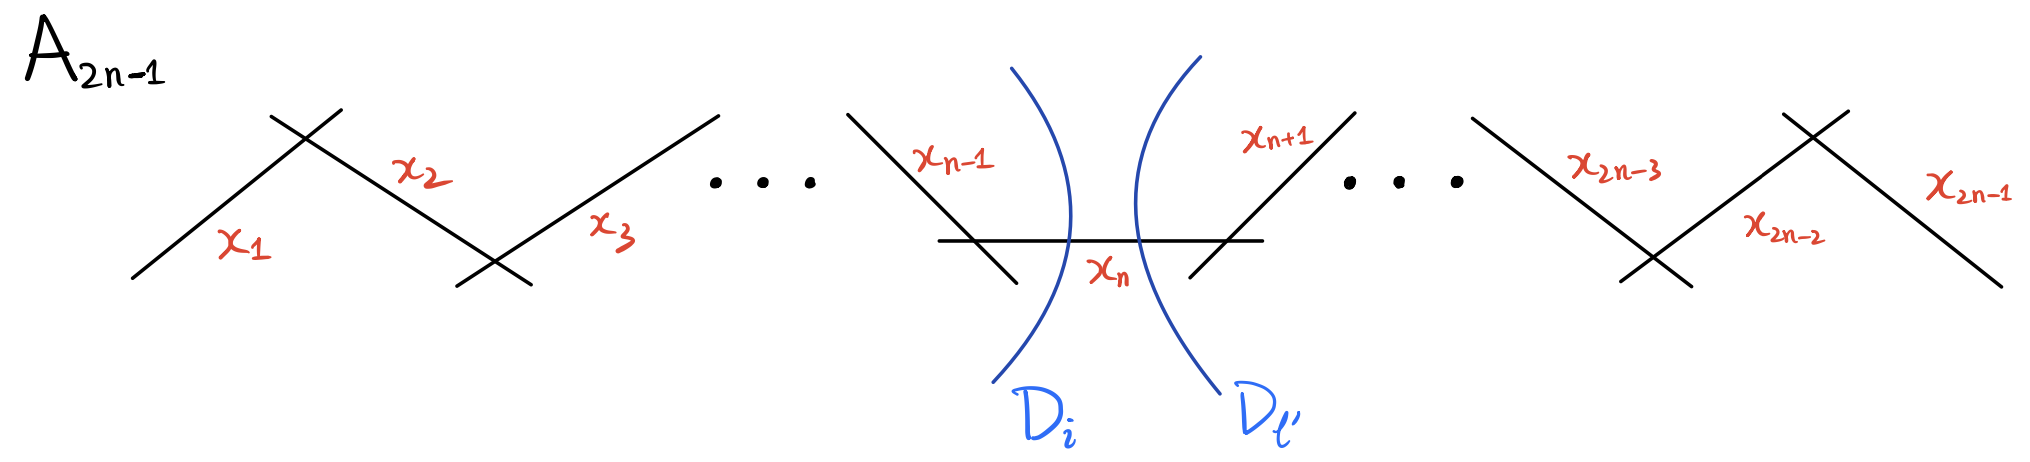
\includegraphics[width=13cm,height=\textheight,keepaspectratio]{A_2n_1.jpg}
\end{minipage}
\caption{Resolution graph of \(A_{2n-1}\)-type}\label{figure:ux20A_2n-1}
\end{figure}

Both \(\beta_i\) and \(\beta_{l'}\) intersect only the middle curve.
Hence the projection of \(\beta_i\) (also \(\beta_{l'}\)) to the root
lattice of type \(A_{2n-1}\) is the fundamental weight \(\lambda_n\).
The weight \(\lambda_n\) can be expressed as
\[\lambda_n = -{1\over 2}x_1 - {2\over 2}x_2 - {3\over 2}x_3 - \cdots - {n\over 2}x_n - {n-1\over 2}x_{n+1} - \cdots - {1\over 2}x_{2n-1},\]
where the coefficients of both \(x_i\) and \(x_{2n-i}\)
\((1\le i\le n)\) are \(-{i\over 2}\). (A general calculation of
fundamental weights can be found in
\cite[PLATE I--X]{bourbaki2002lie4-6}.) This is exactly the projection
of \(\Sigma\) to the associated \(A_{2n-1}\)-root lattice. Thus
\(\Sigma\notin \langle H\rangle\oplus L\).

The cases of types \(D_n\) and \(E_7\) are similar, but a bit more
involved. We call the exceptional curve corresponding to \(m\)-node the
\(m\)-line. See Figure \ref{figure: D_2n-1}, \ref{figure: D_2n},
\ref{figure: E_7} for the numbering of each node.

\begin{figure}
\centering
\begin{minipage}[t]{0.45\linewidth}
\centering
\end{minipage}
\hfill
\begin{minipage}[t]{0.45\linewidth}
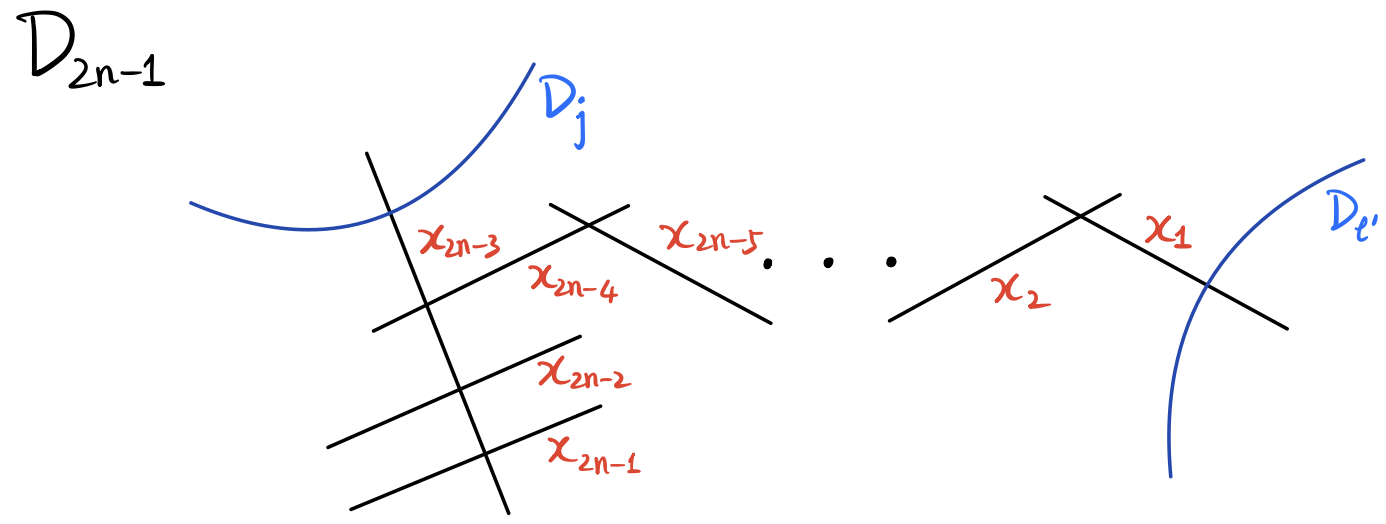
\includegraphics[width=8cm,height=\textheight,keepaspectratio]{D_2n_1.jpg}
\end{minipage}
\caption{Resolution graph of \(D_{2n-1}\)-type}\label{figure:ux20D_2n-1}
\end{figure}

\begin{figure}
\centering
\begin{minipage}[t]{0.45\linewidth}
\centering
\end{minipage}
\hfill
\begin{minipage}[t]{0.45\linewidth}
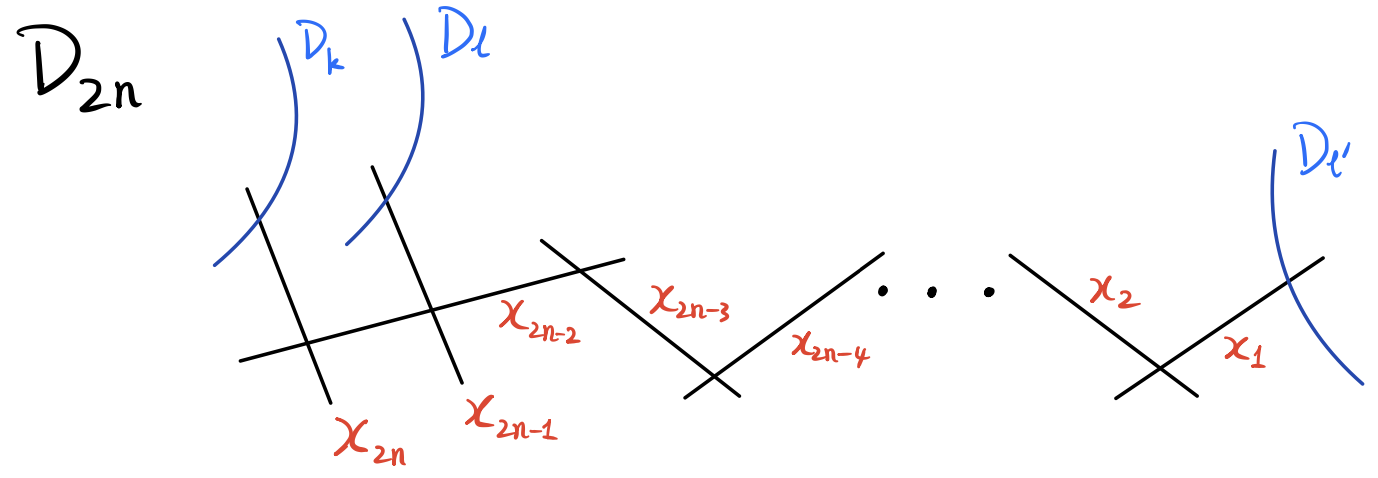
\includegraphics[width=9cm,height=\textheight,keepaspectratio]{D_2n.jpg}
\end{minipage}
\caption{Resolution graph of \(D_{2n}\)-type}\label{figure:ux20D_2n}
\end{figure}

\begin{figure}
\centering
\begin{minipage}[t]{0.45\linewidth}
\centering
\end{minipage}
\hfill
\begin{minipage}[t]{0.45\linewidth}
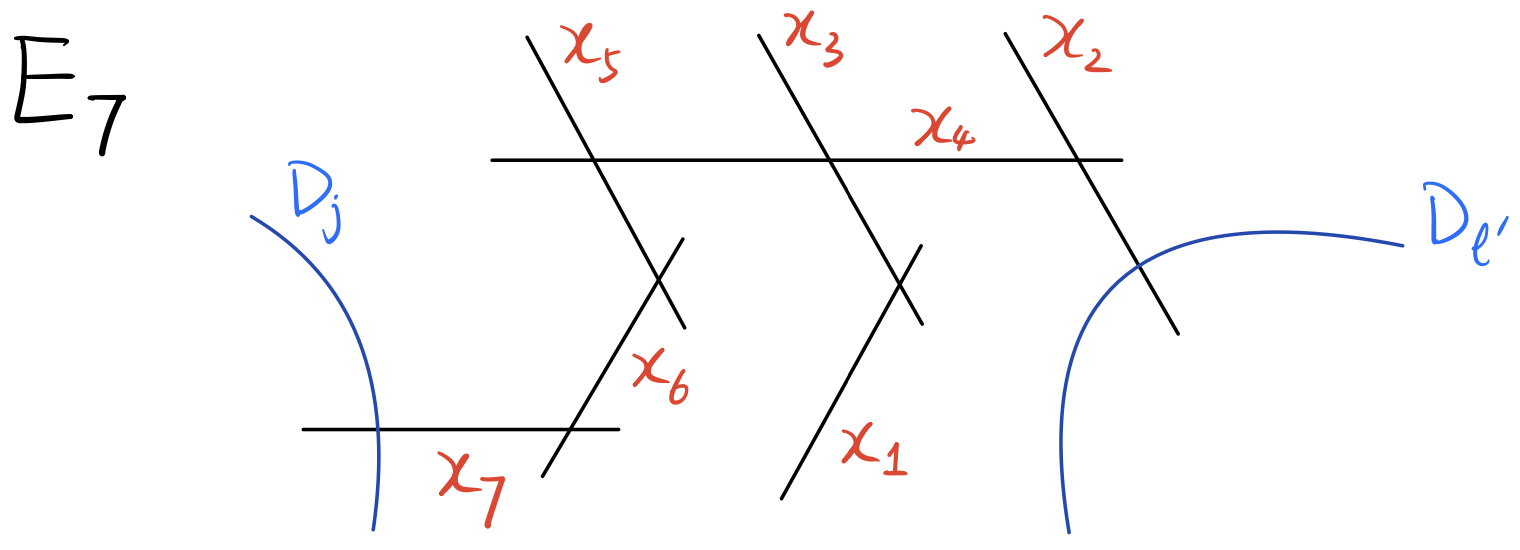
\includegraphics[width=7cm,height=\textheight,keepaspectratio]{E_7.jpg}
\end{minipage}
\caption{Resolution graph of \(E_7\)-type}\label{figure:ux20E_7}
\end{figure}

A singularity of type \(D_{2n-1}\) or \(E_7\) lies on exactly two
irreducible components, which we denote by \(D_j\) and \(D_{l'}\). In
\(D_{2n-1}\) case, the strict transform of the locally cuspidal
component intersects only the \((2n-3)\)-line. The strict transform of
the locally smooth component intersects only the \(1\)-line. The
projection of \(\beta_i\) to the root lattice of type \(D_{2n-1}\) is
the fundamental weight \(\lambda_1\) or \(\lambda_{2n-3}\). The weights
\(\lambda_1\) and \(\lambda_{2n-3}\) have the following expressions
\[\begin{aligned}
    \lambda_{2n-3} &= -x_1-2x_2-3x_3-\cdots-(2n-3)x_{2n-3}-{2n-3\over 2}(x_{2n-2}+x_{2n-1}), \\
    \lambda_{1} &= -(x_1+x_2+\cdots+x_{2n-3})-{1\over 2}(x_{2n-2}+x_{2n-1}).
\end{aligned}\] In \(E_7\) case, the strict transform of the locally
cuspidal component intersects only the \(2\)-line. The strict transform
of the locally smooth component intersects only the \(7\)-line. The
weights \(\lambda_2\) and \(\lambda_7\) have the following expressions
\[\begin{aligned}
    \lambda_{2} &= -{1\over 2}(4x_1+7x_2+8x_3+12x_4+9x_5+8x_6+3x_7), \\
    \lambda_{7} &= -{1\over 2}(2x_1+3x_2+4x_3+6x_4+5x_5+4x_6+3x_7).
\end{aligned}\] These are exactly the projections of \(\Sigma\) to the
associated \(D_{2n-1}\) and \(E_7\). Thus
\(\Sigma\notin \langle H\rangle\oplus L\).

A singularity of type \(D_{2n}\) lies on exactly three irreducible
components, which we denote by \(D_k\), \(D_l\) and \(D_{l'}\). The
strict transform of two components intersect only with the \(2n\)-line
and the \((2n-1)\)-line respectively. The strict transform of the rest
component intersects only the \(1\)-line. The corresponding fundamental
weights can be expressed as \[\begin{aligned}
    \lambda_1 &= -(x_1+x_2+\cdots+x_{2n-2})-{1\over 2}(x_{2n-1}+x_{2n}), \\
    \lambda_{2n-1} &= -{1\over 2}x_1 - {2\over 2}x_2 - {3\over 2}x_3 - \cdots - {2n-2\over 2}x_{2n-2} - {n\over 2}x_{2n-1} - {n-1\over 2}x_{2n}, \\
    \lambda_{2n} &= -{1\over 2}x_1 - {2\over 2}x_2 - {3\over 2}x_3 - \cdots - {2n-2\over 2}x_{2n-2} - {n-1\over 2}x_{2n-1} - {n\over 2}x_{2n}. \\
\end{aligned}\] The strict transform of \(D_{l'}\) may give one or two
components in the resolution graph of the singularity. Every linear
combination of the rest components with coefficients \(0\) or \(1\) has
non-integer coefficients. These are exactly the projections of
\(\Sigma\) to the associated \(D_{2n}\). Thus
\(\Sigma\notin \langle H\rangle\oplus L\).

By the above calculation, any nontrivial \(\mathbb{Z}/2\)-combination of
\(\beta_1,\cdots\beta_{l'-1}\) does not lie in
\(\langle H\rangle\oplus L\). Hence \(\beta_1,\cdots\beta_{l'-1}\) is
\(\mathbb{Z}/2\)-independent in
\(\frac{M^{\iota}}{(\left\langle H \right\rangle\oplus L)^{\iota}}\).~◻

\emph{Remark~ 39}. The above calculation in the case of sextic curves
can also be found in \cite[\S 3, Tabel 1]{yang1996sextic}.

\textbf{Proposition~ 40}. \emph{\label{prop: saturation of M_F} We have
\[\frac{M}{\left\langle H\right\rangle \oplus L}\cong (\mathbb{Z}/2)^{l'-1}.\]
This finite group is generated by equivalence classes of
\(\beta_1,\cdots, \beta_{l'-1}\). Moreover, \(M^{\iota} = P^{\iota}\).}

\emph{Proof.} Since \(\beta_i \in M^{\iota}\) for \(1\le i\le l'\), the
finite-index extensions in
(\ref{eqn: iota-invariant successive saturations}) induces injective
maps of the following finite abelian groups
\[\frac{M^{\iota}}{(\left\langle H \right\rangle\oplus L)^{\iota}} \hookrightarrow \frac{P^{\iota}}{(\left\langle H \right\rangle\oplus L)^{\iota}} \hookrightarrow \frac{P}{\left\langle H \right\rangle\oplus L}.\]
By Lemma \ref{lem: saturation of inv part of P}, we have
\[\frac{M^{\iota}}{(\left\langle H \right\rangle\oplus L)^{\iota}} = \frac{P^{\iota}}{(\left\langle H \right\rangle\oplus L)^{\iota}} \cong (\mathbb{Z}/2)^{l'-1}.\]
By Lemma \ref{lem: Z/2-independence}, there is only one nontrivial
relation among \(\beta_1, \cdots, \beta_{l'}\). This isomorphism implies
that \(M^{\iota} = P^{\iota}\). Moreover, the inclusion
\[\frac{M^{\iota}}{(\left\langle H \right\rangle\oplus L)^{\iota}} \hookrightarrow \frac{M}{\left\langle H \right\rangle\oplus L}\]
is surjective (hence an isomorphism) because
\(\beta_1, \cdots, \beta_{l'}\) lies in \(M^\iota\). We have done.~◻

\textbf{Lemma~ 41}.
\emph{\label{lem: saturation induced by involution, inequality and ADE case}
Let \(L\) be an even lattice and \(\iota\in \mathrm{O}(L)\) be an
involution. Then \(\frac{L}{L^\iota \oplus L^{-\iota}}\) is
\(2\)-elementary, and its cardinality satisfies
\[\bigg|\frac{L}{L^\iota \oplus L^{-\iota}}\bigg| \le 2^{min\{\mathrm{rank} (L^\iota), \mathrm{rank} (L^{-\iota})\}}.\]
In particular, for every root lattice \(L\) of ADE type, the equality is
achieved, i.e.
\[\frac{L}{L^{\iota} \oplus L^{-\iota}} \cong (\mathbb{Z}/2)^{\mathrm{rank} (L^{-\iota})}.\]}

\emph{Proof.} For any \(v\in L\), we have
\(2v = (v+\iota(v))+(v-\iota(v))\), hence
\(2v\in L^{\iota} \oplus L^{-\iota}\). Thus
\(\frac{L}{L^\iota \oplus L^{-\iota}}\) is \(2\)-elementary. Denote by
\(r\coloneqq min\{\mathrm{rank} (L^\iota), \mathrm{rank} (L^{-\iota})\}\).
For any \(n>r\), we assume that there exist
\(\frac{v_1+w_1}{2},\cdots,\frac{v_n+w_n}{2}\) in
\(L\backslash(L^{\iota} \oplus L^{-\iota})\). Without loss of
generality, we assume that
\(\mathrm{rank} (L^\iota) \ge \mathrm{rank} (L^{-\iota})\). Since
\(n > r=\mathrm{rank} (L^{-\iota})\), there exist \(a_1,\cdots,a_n\)
(\(\exists a_i\neq 0\)) such that \(\sum\limits_{i=1}^n a_i w_i = 0\).
Then
\(\sum\limits_{i=1}^n a_i \frac{v_i+w_i}{2} = \sum\limits_{i=1}^n a_i \frac{v_i}{2}\)
lies in \(L^\iota\). Hence \(\sum\limits_{i=1}^n a_i \frac{v_i+w_i}{2}\)
vanishes in \(\frac{L}{L^{\iota} \oplus L^{-\iota}}\), namely, there
exists a nontrivial relation among
\(\frac{v_1+w_1}{2},\cdots,\frac{v_n+w_n}{2}\). Thus
\(\dim_{\mathbb{Z}/2}(\frac{L}{L^\iota \oplus L^{-\iota}}) \le \mathrm{rank} (L^{-\iota})\)
(view \(\frac{L}{L^\iota \oplus L^{-\iota}}\) as a
\(\mathbb{Z}/2\)-vector space).

For root lattices of ADE types, the equality arises from a case-by-case
check. Notice that
\[\bigg|\frac{L}{L^\iota \oplus L^{-\iota}}\bigg|^2 = \frac{|A_{L^\iota} \oplus A_{L^{-\iota}}|}{|A_L|}.\]
For each ADE type, \(A_{L^{-\iota}}\) is listed in Table
\ref{tab: r_R^-}. We list \(A_{L^\iota}\) in Table \ref{tab: r_R^+}.

\centering      

\begin{longtable}[]{@{}ccccc@{}}
\toprule\noalign{}
Root Type \(R\) & \(A_{2n-1}\) & \(A_{2n}\) & \(D_{n}\) (odd) &
\(E_6\) \\
\midrule\noalign{}
\endhead
\bottomrule\noalign{}
\endlastfoot
\(r_R^+\) & \(n\) & \(n\) & \(n-1\) & \(4\) \\
\(A_{R^{-w_0(R)}}\) & \((\mathbb{Z}/2)^{n}\) & \((\mathbb{Z}/2)^n\) &
\((\mathbb{Z}/2)^2\) & \((\mathbb{Z}/2)^2\) \\
\end{longtable}

\label{tab: r_R^+}~◻

\textbf{Proposition~ 42}. \emph{\label{prop: M_F = Z_2-saturation} The
lattice \(M\) is the biggest finite-index extension of
\(P^\iota \oplus L^{-\iota}\) in \(H^2(X,\mathbb{Z})\) such that
\(M\over{P^{\iota}\oplus L^{-\iota}}\) is \(2\)-elementary. Moreover,
\(\frac{M}{P^{\iota}\oplus L^{-\iota}}\cong (\mathbb{Z}/2)^{r^-}\).}

\emph{Proof.} Since \(P^{\iota}\) is a finite-index extension of
\(\left\langle H\right\rangle\oplus L^{\iota}\), \(L^{-\iota}\) is
orthogonal to \(P^{\iota}\) in \(P\). Consider the finite-index
extension \[P^{\iota}\oplus L^{-\iota}\hookrightarrow P.\] By
Proposition \ref{prop: saturation of M_F}, we have
\(M^{\iota} = P^{\iota}\). Thus there is a natural finite-index
extension \[P^{\iota}\oplus L^{-\iota} \hookrightarrow M.\] We have the
following successive finite-index extensions
\[\left\langle H \right\rangle \oplus L^{\iota} \oplus L^{-\iota} \hookrightarrow \left\langle H \right\rangle \oplus L \hookrightarrow M.\]
By Lemma
\ref{lem: saturation induced by involution, inequality and ADE case}, we
have
\(\frac{L}{L^{\iota} \oplus L^{-\iota}} \cong (\mathbb{Z}/2)^{r^-}\). By
Proposition \ref{prop: saturation of M_F}, we have
\(\frac{M}{\left\langle H\right\rangle \oplus L}\cong (\mathbb{Z}/2)^{l'-1}\).
Moreover, we have another successive finite-index extensions
\[\left\langle H \right\rangle \oplus L^{\iota} \oplus L^{-\iota} \hookrightarrow P^{\iota}\oplus L^{-\iota} \hookrightarrow M.\]
By Lemma \ref{lem: saturation of inv part of P} and Proposition
\ref{prop: saturation of M_F}, we have
\(\frac{P^{\iota}}{\left\langle H \right\rangle \oplus L^{\iota}} = \frac{M}{\left\langle H \right\rangle \oplus L} \cong (\mathbb{Z}/2)^{l'-1}\).
It is direct to verify that
\((\left\langle H \right\rangle \oplus L)\cap (P^{\iota}\oplus L^{-\iota}) = \left\langle H \right\rangle \oplus L^\iota \oplus L^{-\iota}\).
Thus
\(\frac{M}{\left\langle H \right\rangle \oplus L^\iota \oplus L^{-\iota}} \cong (\mathbb{Z}/2)^{l'+r^--1}\).
Therefore we conclude
\[\label{eqn: saturation of M over P^iota oplus L^-iota}
        \frac{M}{P^{\iota}\oplus L^{-\iota}}\cong (\mathbb{Z}/2)^{r^-},\]
where \(r^-\) is the sum of all \(r_R^-\) with \(R\) that appear in
\(L\) (with multiplicities).

Since \(P^{\iota}\) is primitive in \(P\), by lattice theory, the
quotient \(\frac{P}{P^{\iota}\oplus L^{-\iota}}\) is isomorphic to
certain subgroup of \(A_{L^{-\iota}}\). By Lemma \ref{lem: anti-inv},
the biggest subgroup of each \(A_{R^{w_0(R)}}\) of the form
\((\mathbb{Z}/2)^k\) is isomorphic to \((\mathbb{Z}/2)^{r_R^-}\). Notice
that \((\mathbb{Z}/2)^{r^-}\) can be naturally decomposed into the
product \(\prod\limits_{R}(\mathbb{Z}/2)^{l_T(R)r_R^-}\). Therefore
\(M\) is the biggest finite-index extension of
\(P^{\iota}\oplus L^{-\iota}\) such that
\(M\over{P^{\iota}\oplus L^{-\iota}}\) is \(2\)-elementary.~◻

\emph{Remark~ 43}. Since \(H\) is primitive in \(H^2(X,\mathbb{Z})\),
\(\frac{P}{\left\langle H \right\rangle \oplus L}\) is a subgroup of
\(A_L\).

\emph{Remark~ 44}. There exist examples such that \(M\) is a proper
sublattice of \(P\), for example, see §\ref{subsec: Zariski pair} and
Propostion \ref{proposition: picard zariski pair}. By
\cite[Proposition 3.4]{yu2023moduli}, \(M=P\) holds for all nodal
singular types. We will give more examples with \(M=P\) in
§\ref{sec: examples and applications}.

\section{Orbifold Structures}\label{sec:ux20orbifoldux20structures}

Given a singular type \(T\), both the moduli space \(\mathcal{M}_T\) and
the associated arithmetic quotient
\(\Gamma_T\backslash(\mathbb{D}_T-\mathcal{H}_T)\) admit natural
orbifold structures induced by their nontrivial automorphism groups. It
is natural to study the relationship of these two orbifold structures.
See \cite{kudla2012occult} and \cite{zheng2021orbifold} for some
well-known cases. In this section, we compare the orbifold structures of
the two sides of the period map
\(\mathscr{P}_T\colon \mathcal{M}_T\to \Gamma_T\backslash(\mathbb{D}_T-\mathcal{H}_T)\).
We follow the setup in §\ref{section: period map}. For a general
introduction to orbifolds, one can see for instance
\cite[Chapter 13]{thurston2022geometry}.

\subsection{A Lattice-theoretic
Criterion}\label{a-lattice-theoretic-criterion}

For \(Z(F)\in \mathbb{P}\mathcal{V}_T\), let \((X_F,H_F,\iota_F)\) be
defined as in §\ref{subsection: ADE K3}, and \(\Delta_F\) be defined as
in §\ref{subsection: define period map}.

\textbf{Proposition~ 45}. \emph{\label{prop: describe Stab_Z(F)} We have
a natural isomorphism \[\begin{aligned}
        \mathrm{Stab}_{Z(F)} &\cong \mathrm{Aut}(X_F,H_F)/\{\mathrm{Id},\iota_F\} \\
        &\cong \mathrm{O}(\Lambda_F,H_F,\Delta_F,H^{2,0}(X_F))/\{\mathrm{Id},\iota_F^*\},
    
\end{aligned}\] where \(\mathrm{Stab}_{Z(F)}\) is the stabilizer of
\(Z(F)\) in \(\mathrm{PGL}(3)\).}

\textbf{Lemma~ 46}. \emph{\label{lem: describe Aut(X_F,H_F,Delta_F)} We
have \[\begin{aligned}
        \mathrm{Aut}(X_F,H_F,\Delta_F) &= \mathrm{Aut}(X_F,H_F) \\
                &\cong \mathrm{O}(\Lambda_F,H_F,\Delta_F,H^{2,0}(X_F)).
    
\end{aligned}\]}

\emph{Proof.} Let \(f\in \mathrm{Aut}(X_F)\) satisfy \(f^*H_F=H_F\).
Then \(f^*L_F=L_F\), as \(L_F\) is the root lattice of
\(\langle H_F,H^{2,0}(X_F)\rangle^\perp_{\Lambda_F}\). Since \(f^*\)
maps effective classes to effective classes, it follows that
\(f^*\Delta_F=\Delta_F\). Consequently, we conclude
\(\mathrm{Aut}(X_F,H_F,\Delta_F) = \mathrm{Aut}(X_F,H_F)\).

Moreover, by the proof of Theorem \ref{theorem: global torelli}, we can
construct an ample class \(\alpha_F\) of \(X_F\) lying in
\(\langle H_F\rangle\oplus L_F\). Since
\(\mathrm{Aut}(X_F,\alpha_F)\cong\mathrm{O}(\Lambda_F,\alpha_F,H^{2,0}(X_F))\)
(given by \(f\mapsto f^*\)) and
\(\mathrm{Aut}(X_F,H_F,\Delta_F) \subset \mathrm{Aut}(X_F,\alpha_F)\),
it follows that \(f\mapsto f^*\) gives
\(\mathrm{Aut}(X_F,H_F,\Delta_F) \cong \\ \mathrm{O}(\Lambda_F,H_F,\Delta_F,H^{2,0}(X_F))\).~◻

\textbf{Lemma~ 47}.
\emph{\label{lem: Aut(Lambda_F,H_F,Delta_F) commutes with iota_F} Each
element \(f\in \mathrm{O}(\Lambda_{F}, \Delta_{F},H_{F})\) commutes with
the involution \(\iota_{F}\).}

\emph{Proof.} Consider a singularity of type \(R\) on \(Z(F)\). The
lattices \(L(R)\) and \(f(L(R))\), both of type \(R\), satisfy
\(f(L(R)\cap \Delta_{F}) = f(L(R))\cap \Delta_{F}\). By Proposition
\ref{prop: iota-action on resolution graph/base} and Remark
\ref{rmk: iota-action on L(R)}, we can identify the generators of
\(L(R)^{\iota_{F}}\) and \(f(L(R))^{\iota_{F}}\). This implies
\(f(L(R)^{\iota_{F}}) = f(L(R))^{\iota_{F}}\). Since \(f(H_{F})=H_{F}\),
we conclude \(f(\Lambda_{F}^{\iota_{F}})=\Lambda_{F}^{\iota_{F}}\).
Consequently, \(f\) commutes with \(\iota_{F}\).~◻

\textbf{Lemma~ 48}. \emph{\label{lem: Aut(X_F,H_F) to Stab_Z(F)} Every
automorphism \(f\in \mathrm{Aut}(X_F,H_F)\) naturally induces an
automorphism of \(Z(F)\subset\mathbb{P}^2\). The only automorphisms of
\(X_F\) inducing the identity map on \(Z(F)\) are the involution
\(\iota_F\) and the identity map.}

\emph{Proof.} By Lemma \ref{lem: describe Aut(X_F,H_F,Delta_F)}, every
\(f\in \mathrm{Aut}(X_F,H_F)\) induces a \(f^*\in\mathrm{O}(\Lambda_F)\)
that preserves \(H_F\) and \(\Delta_F\). Lemma
\ref{lem: Aut(Lambda_F,H_F,Delta_F) commutes with iota_F} ensures that
\(f^*\) commutes with \(\iota_F^*\) on \(\Lambda_F\). By the injectivity
of \(\mathrm{Aut}(X_F)\hookrightarrow\mathrm{O}(\Lambda_F)\), it follows
that \(f\) commutes with \(\iota_F\). Hence \(f\) induces an
automorphism of \(S_F\) that preserves the strict transform of \(Z(F)\),
which lies in the branched locus of \(p_F\colon X_F\to S_F\). Moreover,
since \(f^*H_F=H_F\), \(f\) descends to an automorphism \(\overline{f}\)
of \(\mathbb{P}^2\) that preserves \(Z(F)\).

Let \(f\in\mathrm{Aut}(X_F)\) be an automorphism such that the induced
map \(\overline{f}\) restricts to the identity map on \(Z(F)\). Then
\(\overline{f}\) is the identity map on \(\mathbb{P}^2\). The identity
map lifts trivially to \(S_F\), and thus \(f\) must coincide with either
the identity map on \(X_F\) or the involution \(\iota_F\).~◻

\emph{Proof of Proposition \ref{prop: describe Stab_Z(F)}.} There exists
a natural map
\[\mathrm{Aut}(X_F,H_F) \to \mathrm{Stab}_{Z(F)}, \quad f\mapsto\overline{f}.\]
By Lemma \ref{lem: Aut(X_F,H_F) to Stab_Z(F)}, the kernel of this map is
\(\{\mathrm{Id},\iota_F\}\). Moreover, every automorphism of
\(\mathbb{P}^2\) preserving \(Z(F)\) lifts to an automorphism of the
double cover branched along \(Z(F)\), and subsequently to an
automorphism of \(X_F\). Thus we obtain
\(\mathrm{Stab}_{Z(F)} \cong \mathrm{Aut}(X_F,H_F)/\{\mathrm{Id},\iota_F\}\).

By Lemma \ref{lem: describe Aut(X_F,H_F,Delta_F)}, there is a natural
isomorphism
\[\mathrm{Aut}(X_F,H_F)/\{\mathrm{Id},\iota_F\} \cong \mathrm{O}(\Lambda_F,H_F,\Delta_F,H^{2,0}(X_F))/\{\mathrm{Id},\iota_F^*\}.\]
Combining these results, the proposition follows.~◻

Let \(Z(F_0)\in\mathbb{P}\mathcal{V}_T\) be a base point. By Corollary
\ref{cor: Lambda_F^iota = P_F^iota}, the involution \(\iota_{F_0}\)
induces an action on \(\Lambda_{F_0}\) preserving \(H_{F_0}\) and
\(\Delta_{F_0}\), and acts as \(-\mathrm{Id}\) on \(Q_{F_0}\). We denote
by \(P\Gamma_T\) the quotient group \(\Gamma_T/\{\pm \mathrm{Id}\}\).
The natural map \(\Gamma_T \to \mathrm{Aut}(\mathbb{D}_T)\) descends to
\(P\Gamma_T \hookrightarrow \mathrm{Aut}(\mathbb{D}_T)\). We consider
the orbifold \(P\Gamma_T\backslash(\mathbb{D}_T-\mathcal{H}_T)\) instead
of \(\Gamma_T\backslash(\mathbb{D}_T-\mathcal{H}_T)\). For
\(\omega\in \mathbb{D}_T-\mathcal{H}_T\), the stabilizer of \(\omega\)
in \(P\Gamma_T\) is given by
\[\mathrm{Stab}_\omega = \{ g|_{Q_{F_0}} \,\big|\, g\in \mathrm{O}(\Lambda_{F_0},H_{F_0},\Delta_{F_0}),\, g\cdot\omega=\omega \}/\{\pm \mathrm{Id}\},\]
where \(\omega\) represents a positive complex line in
\(Q_{F_0}\otimes\mathbb{C}\). There exists a
\(Z(F)\in \mathbb{P}\mathcal{V}_T\) satisfying
\(\mathscr{P}_T(Z(F))=[\omega]\). By definition of \(\mathscr{P}_T\),
there exists a path \(\gamma_F\subset\mathbb{P}\mathcal{V}_T\)
connecting \(Z(F)\) and \(Z(F_0)\) such that
\(\gamma_F^*H^{2,0}(X_F)=\omega\). Let \(\varphi\) denote
\(\gamma_F^*\colon H^2(X_F,\mathbb{Z})\to H^2(X_{F_0},\mathbb{Z})\). The
homomorphism \(\varphi\) satisfies \(\varphi(H_F)=H_{F_0}\),
\(\varphi(\Delta_F)=\Delta_{F_0}\). Then we can define a group
homomorphism
\[\mathrm{Aut}(X_F,H_F) \to \{ g|_{Q_{F_0}} \,\big|\, g\in \mathrm{O}(\Lambda_{F_0},H_{F_0},\Delta_{F_0},\omega) \},\quad f \mapsto (\varphi\circ f^*\circ\varphi^{-1})|_{Q_{F_0}},\]
which is surjective. It induces a surjective homomorphism
\(\mathrm{Stab}_{Z(F)}\to\mathrm{Stab}_\omega\).

\textbf{Proposition~ 49}. \emph{\label{prop: orbifold criterion} The
following statements are equivalent to each other.}

\begin{enumerate}
\def\labelenumi{(\roman{enumi})}
\item
  \emph{The period map
  \(\mathscr{P}_T\colon \mathcal{M}_T\to P\Gamma_T\backslash(\mathbb{D}_T-\mathcal{H}_T)\)
  preserves the orbifold structures of the GIT quotient and the
  arithmetic quotient.}
\item
  \emph{The natural restriction map
  \(\mathrm{O}(\Lambda_{F_0},H_{F_0},\Delta_{F_0})\to \Gamma_T\) is an
  isomorphism.}
\item
  \emph{The group \(\mathrm{O}(P_{F_0},H_{F_0},\Delta_{F_0})\) acts
  faithfully on \(A_{P_{F_0}}\).}
\end{enumerate}

\emph{Proof.} The period map \(\mathscr{P}_T\) preserves the orbifold
sturctures if and only if for any
\(\omega\in \mathbb{D}_T-\mathcal{H}_T\) and an associated
\(Z(F)\in \mathbb{P}\mathcal{V}_T\),
\(\mathrm{Stab}_{Z(F)} \cong \mathrm{Stab}_\omega\). By Corollary
\ref{cor: Lambda_F^iota = P_F^iota}, \(\iota_{F_0}\) acts as \(-1\) on
\(Q_{F_0}\), this is equivalent to say that the map
\[\mathrm{Aut}(X_F,H_F)\cong \mathrm{O}(\Lambda_F,H_F,\Delta_F,H^{2,0}(X_F)) \to \{ g|_{Q_{F_0}} \,\big|\, g\in \mathrm{O}(\Lambda_{F_0},H_{F_0},\Delta_{F_0},\omega) \}\]
is an isomorphism. Denote by
\(G_{Z(F)}\coloneqq \mathrm{O}(\Lambda_F,H_F,\Delta_F,H^{2,0}(X_F))\)
and
\(G_\omega\coloneqq \{ g|_{Q_{F_0}} \,\big|\, g\in \mathrm{O}(\Lambda_{F_0},H_{F_0},\Delta_{F_0},\omega) \}\).

By definition, there is a surjective group homomorphism
\(p\colon \mathrm{O}(\Lambda_{F_0},H_{F_0},\Delta_{F_0})\to \Gamma_T\)
defined by restriction. The stabilizer \(G_{Z(F)}\) can be naturally
embedded into \(\mathrm{O}(\Lambda_{F_0},H_{F_0},\Delta_{F_0})\) by the
conjugation of \(\varphi\). Via this embedding, \(G_{Z(F)}\) is
isomorphic to \(p^{-1}(G_\omega)\). Hence \(G_{Z(F)} \cong G_\omega\) is
equivalent to
\(\mathrm{O}(\Lambda_{F_0},H_{F_0},\Delta_{F_0}) \cong \Gamma_T\). The
isomorphism
\(\mathrm{O}(\Lambda_{F_0},H_{F_0},\Delta_{F_0}) \cong \Gamma_T\) is
equivalent to the condition that the identity element (hence every
element) in \(\Gamma_T\) admits a unique lift in
\(\mathrm{O}(\Lambda_{F_0},H_{F_0},\Delta_{F_0})\), which means that
\(\mathrm{O}(P_{F_0},H_{F_0},\Delta_{F_0})\) acts faithfully on
\(A_{P_{F_0}}\).~◻

\subsection{Nodal Singular Types}\label{nodal-singular-types}

As an application, we study the nodal singular types, i.e. the singular
types with only nodes.

\textbf{Proposition~ 50}. \emph{\label{prop: orbi str of nodal types}
The orbifold structures are preserved in all nodal singular types.}

The proposition will be concluded from the following Lemma
\ref{lem: orbi str of irred nodal types} and Lemma
\ref{lem: orbi str of reducible types}.

\textbf{Lemma~ 51}. \emph{\label{lem: orbi str of irred nodal types} For
every irreducible nodal singular type, the orbifold structure is
preserved.}

\emph{Proof.} Let \(r_1,\cdots,r_m\) be the base of
\(L=A_1^{\oplus m}\). We have
\(\mathrm{O}(P,H,\Delta)\cong\mathrm{Aut}(\Delta)\cong\mathfrak{S}_m\)
and \(A_P\cong\mathbb{Z}/2\times(\mathbb{Z}/2)^m\). Moreover,
\(\mathrm{O}(P,H,\Delta)\) acts on \(A_P\) by permuting the \(m\)
generators of the later \(m\) \(\mathbb{Z}/2\)-factors. This action is
faithful.~◻

\textbf{Lemma~ 52}. \emph{\label{lem: 0 or >=5} Fix an arbitrarily nodal
singular type. Let \(r_1,\cdots,r_m\) be the base of
\(L=A_1^{\oplus m}\). For any \(v\in P\) such that
\(v=\mu H+\sum\limits_i \lambda_i r_i\), either all \(\lambda_i\) are
integers, or there exist at least five of \(\lambda_i\) belonging to
\({1\over2}\mathbb{Z}\backslash\mathbb{Z}\).}

\emph{Proof.} For any irreducible nodal singular type, the statement is
followed by \(P=\langle H\rangle\oplus L\).

Consider a reducible nodal singular type. Denote by \(C_1,\cdots,C_l\)
the irreducible components of a sextic curve of the given singular type.
In reducible cases, the statement is equivalent to saying that for any
\(C_{i_1},\cdots,C_{i_k}\) with \(1\le k<l\), \(C_{i_1}+\cdots+C_{i_k}\)
has at least five coefficients relative to \(r_1,\cdots,r_m\) belonging
to \({1\over2}\mathbb{Z}\backslash\mathbb{Z}\).

Each \(C_i\) can be expressed as
\[C_i = {1\over2}(d_i H + \sum_{j\in I_i}r_j),\] where \(d_i=\deg C_i\),
\(I_i\) corresponds to the set of nodes arising from the intersection of
\(C_i\) with the union of other irreducible components. It follows that
\(C_{i_1}+\cdots+C_{i_k}\) satisfies
\[C_{i_1}+\cdots+C_{i_k} \equiv {1\over2}(\sum_{n=1}^k d_{i_n})H + {1\over2}\sum_{j\in I_{i_1,\cdots,i_k}} r_j \mod \langle H\rangle\oplus L,\]
where \(I_{i_1,\cdots,i_k}\) corresponds to the set of nodes arising
from the intersection of \(C_{i_1}\cup\cdots\cup C_{i_k}\) with the
union of other irreducible components. By Bézout theorem, the
cardinality of \(I_{i_1,\cdots,i_k}\) is at least five, thus the lemma
follows.~◻

\textbf{Lemma~ 53}. \emph{\label{lem: orbi str of reducible types} For
every reducible nodal singular type, the orbifold structure is
preserved.}

\emph{Proof.} Let \(g\in\mathrm{O}(P,H,\Delta)\) such that \(g^*\) acts
on \(A_P\) trivially. By Proposition \ref{prop: orbifold criterion}, it
is enough to show \(g=\mathrm{Id}\), namely, \(g\) preserves all
\(r_i, 1\le i\le m\). For each \(r_i\) arising from a self-intersection
node of an irreducible component, \(r_i\) is preserved for the same
reason as in Lemma \ref{lem: orbi str of irred nodal types}. Thus it is
enough to show that each \(r_i\) arising from an intersection of two
irreducible components is preserved. Let \(C,C'\) be two different
irreducible components. Denote by \(J\coloneqq C\cap C'\).

If \(|J|=1\), then both of \(C\) and \(C'\) must be two lines. Denote by
\(r\) the associated exceptional curve. Consider
\({1\over2}(H+r)\in P\otimes\mathbb{Q}\), which is actually an element
in \(P^\vee\). Since \(g^*=\mathrm{Id}\) on \(A_P\), we have
\(g^*[{1\over2}(H+r)]=[{1\over2}(H+r)]=[{1\over2}(H+g r)]\) in \(A_P\),
then \([{1\over2}(r-g r)]=0\) in \(A_P\). If \(g^*r\ne r\), then
\({1\over2}(r-g r)\ne 0\) lies in \(P\), which contradicts to Lemma
\ref{lem: 0 or >=5}.

Consider the case \(|J|\ge 2\). We first assume that for any
\(p_i,p_j\in J\), the associated exceptional curves \(r_i, r_j\) not
form a \(g\)-orbit in \(P\). Consider \({1\over2}(r_i+r_j)\in P^\vee\).
We have
\(g^*[{1\over2}(r_j+r_j)]=[{1\over2}(r_j+r_j)]=[{1\over2}(g r_i+g r_j)]\)
in \(A_P\). If \(g r_i\ne r_i\), then
\({1\over2}(r_i+r_j-g r_i-g r_j)\ne 0\) belongs to \(P\), which
contradicts to Lemma \ref{lem: 0 or >=5}.

Otherwise, there exist \(p_i,p_j\in J\) such that
\(g r_i=r_j, g r_j=r_i\). If \(|J|\ge 3\), then there exists a
\(p_k\in J\backslash\{p_i,p_j\}\). Consider
\({1\over2}(r_i+r_k)\in P^\vee\). Similarly, we have
\({1\over2}(r_i-r_j+r_k-g r_k)\ne 0\) belonging to \(P\). Contradiction.

Otherwise, \(|J|=2\), then \(C,C'\) must be a line and a conic. Then
there exist only three possible cases: one conic plus four lines, two
conics plus two lines and one cubic plus one conic plus one line. Note
that the third case actually contains more than one singular types,
since the cubic could be smooth or nodal. But this is irrelevant to our
discussion.

We can assume that \(C\) is a line and \(C'\) is a conic. Let
\(C\cap C'=\{p_i,p_j\}\) and let \(p_k\) be a node arising from the
intersection of \(C'\) with an irreducible component of odd degree
(which always exists). It is direct to verify that
\({1\over2}(H+r_i+r_k)\in P^\vee\). Then we conclude that
\({1\over2}(r_i-r_j+r_k-g^*r_k)\ne 0\) belongs to \(P\).
Contradiction.~◻

\emph{Remark~ 54}. It is interesting to know whether the orbifold
structures are preserved for other singular types. This question is
still open.

\section{Examples and
Applications}\label{sec:ux20examplesux20andux20applications}

The moduli and period map for nodal singular types have been well
studied, see \cite{yu2023moduli}. In this section, we describe some
further examples as applications.

\subsection{A Quintic Curve with a
Line}\label{a-quintic-curve-with-a-line}

We consider sextic curves that split into a smooth quintic curve and a
line. Let \(V\) denote a complex vector space of dimension \(3\).

\subsubsection{Five Nodes}\label{five-nodes}

Suppose there is no tangent point. Denote the singular type by \(T_0\).
This case is first studied by Laza \cite{laza2009deformations}, and is
related to the study of the minimal-elliptic surface singularity
\(N_{16}\). This case is also included in \cite{yu2023moduli}.

In this case, \(\mathcal{V}_{T_0}\) consists of pairs
\((F_5,F_1)\in \mathrm{Sym}^5 V^*\times V^*\) such that \(Z(F_5)\) and
\(Z(F_1)\) have five different intersection points. It is direct
\(\dim \mathcal{M}_{T_0}=14\), which coincides with the expected
dimension. The normalization \(\widehat{\mathbb{P}\mathcal{V}}_{T_0}\)
of \(\mathbb{P}\overline{\mathcal{V}}_{T_0}\) is given by
\(\mathbb{P}(\mathrm{Sym}^5 V^*) \times \mathbb{P}(V^*)\), see
\cite[\S 4.2]{yu2023moduli}.

For any fixed \(F\in\mathcal{V}_{T_0}\), we have
\(L_F\cong A_1^{\oplus 5}\). Denote \(\Delta_F\) by
\(\{ e_1,\cdots,e_5 \}\). Corollary \ref{cor: if only A_1,D_2n,E_7,E_8}
implies \(P_F=P_F^{\iota}\). By Proposition
\ref{prop: saturation of M_F}, we have:

\textbf{Proposition~ 55}. \emph{The lattice \(P_F\) is generated by
\(\langle H\rangle\oplus L_F\) and \({H-e_1-\cdots-e_5\over2}\).}

\emph{Remark~ 56}. For a generic \(F\in\mathcal{M}_{T_0}\), the K3
surface \(X_F\) admits an elliptic fibration without sections (it admits
a bi-section). This fibration has \(1\) type \(I_0^*\) fiber and \(18\)
nodal fibers. The lattice \(P_F\) is isomorphic to \(U(2)\oplus D_4\).
The Picard lattice of the associated Jacobian elliptic K3 surface is
\(U\oplus D_4\), and the Mordell--Weil group is trivial. This example
also appears in \cite[Table 1.1, No. 6]{belcastro2002picard} and
\cite[Table 2]{clingher2024neron-severi}.

Recall that \(Q_F\coloneqq P_F^\perp\), and
\(Q_F\cong U(2)\oplus U\oplus D_4\oplus E_8\). The associated period
domain is \(\mathbb{D}_{T_0}\coloneqq\mathbb{D}(Q_F)\), which is a type
IV domain of dimension \(14\). The associated arithmetic group
\(\Gamma_{T_0}\) has the following expression
\[\Gamma_{T_0} = \{ g\in\mathrm{O}(Q_F) \,|\, g \textup{ acts on } A_{Q_F} \textup{ through the } \mathfrak{S}_5\textup{-action on } A_{P_F}  \},\]
where \(\mathfrak{S}_5\)-action permutes \(e_1,\cdots,e_5\).

The hyperplane arrangement \(\mathcal{H}_{T_0}^*\) is empty. Thus
\(\mathscr{P}_{T_0}\) extends to an isomorphism
\(\mathcal{M}_{T_0}^{\mathrm{ADE}}\cong \Gamma_{T_0}\backslash\mathbb{D}_{T_0}\),
see \cite[Theorem 4.1]{laza2009deformations} and
\cite[Proposition 3.7]{yu2023moduli}\footnote{There is a small typo in
  \cite[Proposition 3.7]{yu2023moduli}: "\(\Sigma_T\)" should be revised
  as "\(\overline{\Sigma}_T\)", the closure of \(\Sigma_T\) in the GIT
  compactification. This criterion holds for all ADE singular types.}.
The Looijenga compactification with respect to the empty hyperplane
arrangement is exactly the Baily--Borel compactification. Hence the
period map \(\mathscr{P}_{T_0}\) extends to an isomorphism
\(\overline{\mathcal{M}}_{T_0}\cong \overline{\Gamma_{T_0}\backslash\mathbb{D}_{T_0}}^{\mathrm{bb}}\),
also see \cite[Theorem 4.2]{laza2009deformations} and
\cite[Proposition 4.3]{yu2023moduli}.

By Proposition \ref{prop: orbi str of nodal types}, the period map
\(\mathscr{P}_{T_0}\) induces an isomorphism of \(\mathcal{M}_{T_0}\)
and \(P\Gamma_{T_0}\backslash(\mathbb{D}_{T_0}-\mathcal{H}_{T_0})\) as
orbifolds.

\subsubsection{One Tacnode and Three
Nodes}\label{one-tacnode-and-three-nodes}

Suppose that there is one tacnode and three nodes. Denote the singular
type by \(T_1\). Let \(\mathcal{V}_{5}\) consist of
\(F_5\in\mathrm{Sym}^5 V^*\) such that \(Z(F_5)\) is a smooth quintic
curve. In this case, \(\mathbb{P}\mathcal{V}_{T_1}\) is a Zariski open
subset of the universal family over \(\mathcal{U}_{5,1}\).

We construct \(\widehat{\mathbb{P}\mathcal{V}}_{T_1}\) as follows.
Define \(G_1\) as \(\{ 
(L,x)\in\mathbb{P}(V^*)\times\mathbb{P}(V) \,|\, x\in Z(L) \}\), which
is a smooth \(\mathbb{P}^1\)-bundle on \(\mathbb{P}(V^*)\). Define
\(G_{T_1}\) as
\[\{ (L,x,F)\in G_1\times\mathbb{P}(\mathrm{Sym}^5 V^*) \,|\, x\in Z(F),\, \mathrm{mult}_x(Z(F)\cdot Z(L))\ge 2 \}.\]
The space \(G_{T_1}\) is a smooth \(\mathbb{P}^{18}\)-bundle on \(G_1\).

\textbf{Proposition~ 57}.
\emph{\label{prop: normalization for quintic plus 1 tangent} The
normalization space \(\widehat{\mathbb{P}\mathcal{V}}_{T_1}\) is
isomorphic to \(G_{T_1}\).}

\emph{Proof.} Let \(\mathcal{U}\) be the subspace of
\(\mathbb{P}(V^*)\times\mathbb{P}(V)\times\mathbb{P}(\mathrm{Sym}^5 V^*)\)
defined by \[\{ (L,x,F) \,|\, x\in Z(L)\cap Z(F) \}.\] The natural
morphism \(G_{T_1}\to \mathbb{P}(\mathrm{Sym}^6 V^*)\) factors through
the following morphisms
\[G_{T_1} \to \mathcal{U} \to \mathbb{P}(V^*)\times\mathbb{P}(\mathrm{Sym}^5 V^*) \to \mathbb{P}(\mathrm{Sym}^6 V^*).\]
The first map is a natural inclusion, the second map is finite
surjective and of degree \(5\), and the last map is finite and
generically injective. Notice that
\(G_{T_1}\to \mathbb{P}(\mathrm{Sym}^6 V^*)\) is generically injective.
Therefore, \(G_{T_1}\to \mathbb{P}(\mathrm{Sym}^6 V^*)\) is finite and
generically injective. Its image contains
\(\mathbb{P}\mathcal{V}_{T_1}\) as a Zariski open subset, and thus
equals \(\mathbb{P}\overline{\mathcal{V}}_{T_1}\). Therefore,
\(G_{T_1}\) is the normalization of
\(\mathbb{P}\overline{\mathcal{V}}_{T_1}\).~◻

For any fixed \(F\in\mathcal{V}_{T_1}\), we have
\(L_F\cong A_3\oplus A_1^{\oplus 3}\). Denote by
\(\{\epsilon_1,\epsilon_2,\epsilon_3\}\) the effective base of \(A_3\)
and by \(e_1,e_2,e_3\) the effective bases of the three copies of
\(A_1\). Then \(\Delta_F\) is given by
\(\{ \epsilon_1,\epsilon_2,\epsilon_3;e_1;e_2;e_3 \}\).

\textbf{Lemma~ 58}.
\emph{\label{lem: 1 A_3 + 3 A_1: L_F^-iota = P_F^-iota} We have
\(L_F^{-\iota} = P_F^{-\iota}\).}

\emph{Proof.} By definition, \(L_F^{-\iota}\) is generated by
\(\epsilon_1-\epsilon_3\), where \((\epsilon_1-\epsilon_3)^2=-4\). Since
\(({\epsilon_1-\epsilon_3\over2})^2=-1\) and \(P_F\) is even,
\(L_F^{-\iota}\) does not admit any further finite-index extension in
\(P_F\), namely \(L_F^{-\iota} = P_F^{-\iota}\).~◻

Recall that \(M_F\) denotes the lattice generated by
\(\langle H_F\rangle\oplus L_F\) and
\(u\coloneqq{H-(2\epsilon_2+\epsilon_1+\epsilon_3)-e_1-e_2-e_3\over2}\).

\textbf{Proposition~ 59}. \emph{\label{prop: 1 A_3 + 3 A_1: P=M} We have
\(P_F=M_F\).}

\emph{Proof.} It is direct to check that there exists a decomposition of
\(M_F\) as following
\[M_F = \langle H_F-e_2,H_F-e_3 \rangle \oplus \langle e_1,u,\epsilon_2,\epsilon_1,\epsilon_3 \rangle \cong U(2)\oplus D_5.\]
Thus we have \(A_{M_F}\cong (\mathbb{Z}/2)^2\times\mathbb{Z}/4\). By
Lemma \ref{lem: 1 A_3 + 3 A_1: L_F^-iota = P_F^-iota} and Proposition
\ref{prop: saturation of M_F}, the quotient
\(P_F\over{M_F^\iota\oplus M_F^{-\iota}}\) is isomorphic to a subgroup
of \(A_{M_F^\iota}\) and also a subgroup of \(A_{M_F^{-\iota}}\). Since
\(A_{M_F^\iota}\cong(\mathbb{Z}/2)^4\) and
\(A_{M_F^{-\iota}}\cong\mathbb{Z}/4\),
\(P_F\over{M_F^\iota\oplus M_F^{-\iota}}\) is a subgroup of
\(\mathbb{Z}/2\). Moreover, we have
\({M_F\over{M_F^\iota\oplus M_F^{-\iota}}}\cong\mathbb{Z}/2\). By
definition, \(M_F\subset P_F\), thus \(M_F=P_F\).~◻

\emph{Remark~ 60}. For a generic \(F\in\mathcal{M}_{T_1}\), the K3
surface \(X_F\) admits an elliptic fibration \(\pi_1\) with sections.
This fibration has a type \(I_0^*\) fiber and \(18\) nodal fibers. The
Mordell--Weil group of \(\pi_1\) is of rank \(1\) and torsion-free.

\emph{Remark~ 61}. For a generic \(F\in\mathcal{M}_{T_1}\), \(X_F\) also
admits an elliptic fibration \(\pi_2\) without sections (it admits a
bi-section). This fibration has a type \(I_1^*\) fiber and \(17\) nodal
fibers. The Jacobian elliptic surface of \(\pi_2\) has Picard lattice
isomorphic to \(U\oplus D_5\). The Mordell--Weil group is trivial.

We have \(Q_F\cong U\oplus U(2)\oplus A_3\oplus E_8\). The period domain
\(\mathbb{D}_{T_1}\) is a type IV domain of dimension \(13\). The
arithmetic group \(\Gamma_{T_1}\) can be expressed as
\[\Gamma_{T_1} = \{ g\in\mathrm{O}(Q_F) \,|\, g \textup{ acts on } A_{Q_F} \textup{ through the } \mathfrak{S}_2\times\mathfrak{S}_3\textup{-action on } A_{P_F} \},\]
where \(\mathfrak{S}_2\)-action (respectively,
\(\mathfrak{S}_3\)-action) permutes \(\epsilon_1,\epsilon_3\)
(respectively, \(e_1,e_2,e_3\)). By
\cite[Proposition 3.7]{yu2023moduli}, the hyperplane arrangement
\(\mathcal{H}_{T_1}^*\) is empty. The period map \(\mathscr{P}_{T_1}\)
extends to an isomorphism
\(\mathcal{M}_{T_1}^{\mathrm{ADE}}\cong\Gamma_{T_1}\backslash\mathbb{D}_{T_1}\)
and further an isomorphism
\(\overline{\mathcal{M}}_{T_1}\cong \overline{\Gamma_{T_1}\backslash\mathbb{D}_{T_1}}^{\mathrm{bb}}\).

\subsubsection{Two Tacnodes and One
Node}\label{two-tacnodes-and-one-node}

Suppose there are two tangent points. Denote the singular type by
\(T=T_2\). Due to a classical result by Schubert
\cite{schubert1879kalkul}, a generic smooth degree \(d\) plane curve has
\(d(d-2)(d^2-9)\over2\) bitangents. Thus a generic smooth plane quintic
curve has \(120\) bitangents. Denote by \(\mathcal{M}_5\) the moduli
space of smooth quintic curves. The natural projection
\(\mathcal{M}_{T_2}\to \mathcal{M}_5\) is a finite morphism of degree
\(120\).

We construct \(\widehat{\mathbb{P}\mathcal{V}}_{T_2}\) as follows.
Define \(\widetilde{G}_1\) as
\(\{ (L,x,y)\in\mathbb{P}(V^*)\times\mathbb{P}(V)\times\mathbb{P}(V) \,|\, x,y\in Z(L) \}\),
which is a smooth \(\mathbb{P}^1\times\mathbb{P}^1\)-bundle on
\(\mathbb{P}(V^*)\). The total space \(\widetilde{G}_1\) admits an
(fiberwise) involution \(\tau\) defined by switching \(x\) and \(y\).
Define \(G_1\coloneqq \widetilde{G}_1/\tau\). Since the fixed locus of
\(\tau\) has codimension \(1\) in \(\widetilde{G}_1\), \(G_1\) is
smooth. In fact, it is a \(\mathbb{P}^2\)-bundle on \(\mathbb{P}(V^*)\).
Denote by \([L,x,y]\) the image of \((L,x,y)\in\widetilde{G}_1\) in
\(G_1\). Define \(G_{T_2}\) as
\[\{ ([L,x,y],F)\in G_1\times\mathbb{P}(\mathrm{Sym}^5 V^*) \,|\, x,y\in Z(F),\, Z(F)\textup{ satisfies }(\star) \},\]
where the condition \((\star)\) means: when \(x\ne y\),
\(\mathrm{mult}_x (Z(F)\cdot Z(L))\ge 2\) and
\(\mathrm{mult}_y (Z(F)\cdot Z(L))\ge 2\); when \(x=y\),
\(\mathrm{mult}_x(Z(F)\cdot Z(L))\ge 4\). It is a smooth
\(\mathbb{P}^{16}\)-bundle on \(G_1\). Similarly to Proposition
\ref{prop: normalization for quintic plus 1 tangent}, we can describe
the normalization of \(\mathbb{P}\overline{\mathcal{V}}_{T_2}\) as
follows.

\textbf{Proposition~ 62}. \emph{The normalization space
\(\widehat{\mathbb{P}\mathcal{V}}_{T_2}\) is isomorphic to \(G_{T_2}\).}

For any fixed \(F\in\mathcal{M}_{T_2}\), we have
\(L_F\cong A_3^{\oplus 2}\oplus A_1\). Denote by \((\epsilon_i)_i\) and
\((\delta_i)_i\) the effective bases of two copies of \(A_3\)
respectively, and by \(e\) the effective base of \(A_1\). Then
\(\Delta_F\) is given by
\(\{ \epsilon_1,\epsilon_2,\epsilon_3;\delta_1,\delta_2,\delta_3;e \}\).

\textbf{Lemma~ 63}. \emph{\label{lem: 2 A_3 + 1 A_1: L^-iota = P^-iota}
We have \(L_F^{-\iota}=P_F^{-\iota}\).}

\emph{Proof.} By definition, \(L_F^{-\iota}\) is generated by
\(\epsilon_1-\epsilon_3\) and \(\delta_1-\delta_3\). The only possible
value for \((a,b)\) \((0\le a,b\le 3)\) that results in
\(a(\epsilon_1-\epsilon_3)+b(\delta_1-\delta_3)\over4\) having an even
self-intersection number is \((a,b)=(2,2)\). However,
\((\epsilon_1-\epsilon_3)+(\delta_1-\delta_3)\over2\) is a root that is
orthogonal to \(H_F\), so it does not belong to \(P_F\). Thus
\(L_F^{-\iota}\) does not admit any further finite-index extension in
\(P_F\), namely \(L_F^{-\iota} = P_F^{-\iota}\).~◻

In this case, \(M_F\) is generated by \(\langle H_F\rangle\oplus L_F\)
and
\(u\coloneqq {H_F-(2\epsilon_2+\epsilon_1+\epsilon_3)-(2\delta_2+\delta_1+\delta_3)-e\over2}\).

\textbf{Proposition~ 64}. \emph{We have
\(M_F \cong \langle -4 \rangle\oplus U\oplus D_5\).}

\emph{Proof.} It is easy to check \(A_{M_F}\cong(\mathbb{Z}/4)^2\),
which is generated by
\({H\over2}+{3\epsilon_1+2\epsilon_2+\epsilon_3\over4}\) and
\({e\over2}+{3\delta_1+2\delta_2+\delta_3\over4}\). By
\cite[Chapter 15, \S 7.4]{conway1999sphere}, we have
\(A_{M_F}\cong 4^{-2}_{2}\) (Conway--Sloane symbol). By
\cite[Cor 1.13.3]{nikulin1979integer}, there exists a unique \(N\) (up
to isomorphism) of signature \((1,7)\) such that
\(A_N\cong 4^{-2}_{2}\). It is direct to verify that the discriminant
form of \(\langle -4 \rangle\oplus U\oplus D_5\) is isomorphic to
\(A_N\cong 4^{-2}_{2}\).~◻

\textbf{Proposition~ 65}. \emph{We have \(P_F=M_F\).}

\emph{Proof.} It is clear that \(A_{M_F^\iota}\cong(\mathbb{Z}/2)^4\).
By Lemma \ref{lem: 2 A_3 + 1 A_1: L^-iota = P^-iota},
\(A_{M_F^{-\iota}}\cong(\mathbb{Z}/4)^2\). By a parallel argument in the
proof of Proposition \ref{prop: 1 A_3 + 3 A_1: P=M}, we can conclude
\(P_F=M_F\).~◻

\emph{Remark~ 66}. For a generic \(F\in\mathcal{V}_T\), the K3 surface
\(X_F\) admits an elliptic fibration \(\pi_1\) with sections. There
exists a type \(I_1^*\) fiber and \(17\) nodal fibers. The Mordell--Weil
group is of rank one and torsion-free.

We have \(Q_F\cong \langle 4\rangle\oplus A_3\oplus U\oplus E_8\). The
arithmetic group \(\Gamma_{T_2}\) can be described as
\[\Gamma_{T_2} = \{ g\in\mathrm{O}(Q_F) \,|\, g \textup{ acts on } A_{Q_F} \textup{ through the } (\mathfrak{S}_2)^2\times\mathfrak{S}_2\textup{-action on } A_{P_F} \},\]
where the first two \(\mathfrak{S}_2\)-actions permute
\(\epsilon_1,\epsilon_3\) and \(\delta_1,\delta_3\) respectively, and
the last \(\mathfrak{S}_2\)-action permutes the two sets
\(\{\epsilon_i\}\) and \(\{\delta_i\}\). Analogously to the previous
cases, the period map \(\mathscr{P}_{T_2}\) extends first to an
isomorphism
\(\mathcal{M}_{T_2}^{\mathrm{ADE}} \cong \Gamma_{T_2} \backslash \mathbb{D}_{T_2}\)
and then further to
\(\overline{\mathcal{M}}_{T_2} \cong \overline{\Gamma_{T_2} \backslash \mathbb{D}_{T_2}}^{\mathrm{bb}}\).

\subsection{A Quartic Curve with Two
Bitangents}\label{a-quartic-curve-with-two-bitangents}

The nodal case of quartic curves with two lines is discussed in
\cite{gallardo2018compactifications}. We consider the singular type
\(T\) when the two lines are both bitangents. Each smooth quartic curve
admits \(28\) bitangents. Let \(\mathcal{M}_4\) denote the moduli space
of quartic curves. The natural projection
\(\mathcal{M}_T\to \mathcal{M}_4\) is a finite morphism of degree
\(\binom{28}{2}\).

For any fixed \(F\in\mathcal{V}_{T}\), we have
\(L_F\cong A_1\oplus A_3^{\oplus 4}\). Denote by
\(\Delta\coloneqq \{ e;\alpha_1,\alpha_2,\alpha_3;\beta_1,\beta_2,\beta_3;\\ \epsilon_1,\epsilon_2,\epsilon_3;\delta_1,\delta_2,\delta_3 \}\).
In this case, \(M_F\) is generated by \(\langle H\rangle \oplus L\),
\(u\coloneqq{H-e-(2\alpha_2+\alpha_1+\alpha_3)-(2\beta_2+\beta_1+\beta_3)\over2}\)
and
\(v\coloneqq{H-e-(2\epsilon_2+\epsilon_1+\epsilon_3)-(2\delta_2+\delta_1+\delta_3)\over2}\).

\textbf{Lemma~ 67}. \emph{We have \(M_F^{-\iota}=P_F^{-\iota}\).}

\emph{Proof.} Let
\(w\coloneqq{a(\alpha_1-\alpha_3)+b(\beta_1-\beta_3)+c(\epsilon_1-\epsilon_3)+d(\delta_1-\delta_3)\over4}\)
be an element in \((A_3^{\oplus4})^\vee\), where \(0\le a,b,c,d\le 3\).
If \([w]\) is an isotropic element in \(A_{A_3^{\oplus4}}\), then we
have \(8\,|\,a^2+b^2+c^2+d^2\). Then either \((a,b,c,d)\) has two
entries equal to \(2\) and two to \(0\), or \((a,b,c,d)\) is equal to
\((2,2,2,2)\). In the former case, all the entries correspond to roots
orthogonal to \(H_F\), none of which lies in \(P_F\). The element
corresponding to \((2,2,2,2)\) is contained in \(M_F^{-\iota}\).~◻

\textbf{Question~ 68}. \emph{Do we have \(P_F=M_F\)?}

\emph{Remark~ 69}. Since \(A_{M_F^{\iota}}\cong(\mathbb{Z}/2)^6\) and
\(A_{M_F^{-\iota}}\cong(\mathbb{Z}/4)^2\times(\mathbb{Z}/2)^2\), there
may exist a finite-index extension
\(M_F^{\iota}\oplus M_F^{-\iota}\hookrightarrow P\) such that
\({P\over M_F^{\iota}\oplus M_F^{-\iota}}\cong(\mathbb{Z}/2)^4\). Notice
that \({M_F\over M_F^{\iota}\oplus M_F^{-\iota}}\cong(\mathbb{Z}/2)^3\).
There may not be an easy way to decide whether \(P_F=M_F\).

\emph{Remark~ 70}. For a generic \(F\in\mathcal{M}_T\), \(X_F\) admits
an elliptic fibration \(\pi_1\) with sections. There exists a type
\(I_1^*\) fiber, \(2\) type \(I_4\) fibers and \(15\) nodal fibers.

\emph{Remark~ 71}. For a generic \(F\in\mathcal{M}_T\), \(X_F\) admits
another elliptic fibration without sections (it admits a bi-section).
There exist \(2\) type \(I_2^*\) fibers and \(10\) nodal fibers.

The arithmetic group \(\Gamma_{T}\) can be characterized as
\[\Gamma_{T} = \{ g\in\mathrm{O}(Q_F) \,|\, g \textup{ acts on } A_{Q_F} \textup{ through the } (\mathfrak{S}_2)^4\times\mathfrak{S}_4\textup{-action on } A_{P_F} \},\]
where the four \(\mathfrak{S}_2\)-actions permutes
\(\alpha_1,\alpha_3\); \(\beta_1,\beta_3\); \(\epsilon_1,\epsilon_3\)
and \(\delta_1,\delta_3\) respectively, and the
\(\mathfrak{S}_4\)-action permutes the four sets \(\{\alpha_i\}\),
\(\{\beta_i\}\), \(\{\epsilon_i\}\) and \(\{\delta_i\}\). Following the
same argument, \(\mathscr{P}_{T}\) extends to an isomorphism
\(\mathcal{M}_{T}^{\mathrm{ADE}} \cong \Gamma_{T} \backslash \mathbb{D}_{T}\)
and further to
\(\overline{\mathcal{M}}_{T} \cong \overline{\Gamma_{T} \backslash \mathbb{D}_{T}}^{\mathrm{bb}}\).

The moduli space of quartic curves admits an occult period map to an
arithmetic ball quotient dimension \(6\), see \cite{kondo2011moduli}. A
smooth quartic curve is a Riemann surface of genus three. Its Jacobian
is a principal polarized abelian variety of dimension three. This leads
to a birational equivalence between the moduli space of quartic curves
and an arithmetic quotient of the Siegel upper half-space
\(\mathcal{S}_3\) of degree \(3\). It would be interesting to study more
relations among the three arithmetic quotients of different types and
their compactifications.

\subsection{Zariski Pairs}\label{subsec:ux20Zariskiux20pair}

These examples had been discussed in
\cite[\S 3]{yang2012discriminantal}. We present a construction of them
from a more geometric viewpoint.

A pair of reduced plane curves of the same degree, which have the same
combinatorial type of singularities but are not equisingular deformation
equivalent, is usually called \emph{Zariski pairs}. Zariski showed that
the space of irreducible sextic curves with six cusps as the only
singularities form at least two irreducible components, which provided
the first example, see \cite{zariski1931irregularity}. Degtyarev showed
that they actually form exactly two irreducible components, see
\cite[Theorem 5.3.2]{degtyarev2008deformations}. Both of the two
irreducible components are smooth of the same expected dimension.

Denote by \(T_1,T_2\) the two corresponding singular types, where
\(T_2\) corresponds to sextic curves whose six cusps lie on a conic.

Let \(C\) be a sextic of \(T_2\)-type. Denote by \(D\) for the conic
containing the six cusps \(p_1,\cdots,p_6\) of \(C\). By Bézout theorem,
\(D\cap C = \{ p_1,\cdots,p_6 \}\) and the intersection multiplicity of
each \(p_i\) is two. Let \(f\colon S\to \mathbb{P}^2\) be the blowup of
\(\{ p_1,\cdots,p_6 \}\) on \(\mathbb{P}^2\), and denote by
\(E_1,\cdots,E_6\) the exceptional curves. We still denote by \(C\)
(respectively, \(D\)) the strict transform of \(C\) (respectively,
\(D\)). Then \(C\) and \(D\) are disjoint in \(S\). For each
\(1\le i\le 6\), we have \(E_i^2=-1\) and \(E_i\cdot D=1\).

Let \(\pi\colon X\to S\) be the double cover branched over \(C\). Then
\(\pi^{-1}(D)\) is a disjoint union of \(D_1\) and \(D_2\), where
\(D_1,D_2\) are both isomorphic to \(D\). Moreover, we have
\(\pi^* E_i = \widetilde{E}_i + \widetilde{F}_i\) and
\(\pi^* C = 2 \widetilde{C}\), where each
\((\widetilde{E}_i,\widetilde{F}_i)\) forms a \(A_2\)-type Dynkin
diagram, \(\widetilde{C}\) is reduced and
\(\widetilde{E}_i\cdot \widetilde{C} = \widetilde{F}_i\cdot \widetilde{C} = 1\).
Let \(H\) be the pullback of the hyperplane class on \(\mathbb{P}^2\).
We have \(H^2=2\) and \(H\cdot D_i=2\). It is direct to verify that
\[D_1 = H - \frac{1}{3}\sum_{i=1}^6 (2 \widetilde{E}_i + \widetilde{F}_i),\quad D_2 = H - \frac{1}{3}\sum_{i=1}^6 (\widetilde{E}_i + 2 \widetilde{F}_i).\]
It is clear that neither \(D_1\) nor \(D_2\) lies in
\(\left\langle H\right\rangle \oplus L\).

Due to the classification by Zariski and Degtyarev, we have the
following:

\textbf{Proposition~ 72}.
\emph{\label{proposition: picard zariski pair}}

\begin{enumerate}
\def\labelenumi{(\roman{enumi})}
\item
  \emph{For the \(T_1\)-type, the generic Picard group \(P_{T_1}\) of
  the associated K3 surfaces is generated by \(H\) and \(L\).}
\item
  \emph{For the \(T_2\)-type, the generic Picard group \(P_{T_2}\) of
  the associated K3 surfaces is generated by \(H\), \(L\) and \(D_1\).}
\end{enumerate}

The singular type \(T_2\) provides an example for \(P\ne M\).

We have
\(Q_{T_1}=P_{T_1}^\perp\cong \langle -2\rangle\oplus U(3)^{\oplus 2}\oplus A_2^{\oplus 2}\),
\(Q_{T_2}=P_{T_2}^\perp\cong \langle -2\rangle\oplus U\oplus U(3)\oplus A_2^{\oplus 2}\).
Both of the period domains \(\mathbb{D}_{T_1}\) and \(\mathbb{D}_{T_2}\)
are type IV domains of dimension \(7\). The arithmetic group
\(\Gamma_{T_1}\) can be written in the form of
\[\Gamma_{T_1} = \{ g\in\mathrm{O}(Q_{T_1}) \,|\, g \textup{ acts on } A_{Q_{T_1}} \textup{ through the } (\mathfrak{S}_2)^6\times\mathfrak{S}_6\textup{-action on } A_{P_{T_1}} \}.\]
Similar for the arithmetic group \(\Gamma_{T_2}\),
\[\Gamma_{T_2} = \{ g\in\mathrm{O}(Q_{T_2}) \,|\, g \textup{ acts on } A_{Q_{T_2}} \textup{ through the } (\mathfrak{S}_2)^4\times\mathfrak{S}_4\textup{-action on } A_{P_{T_2}} \}.\]
For \(i=1,2\), the period map \(\mathscr{P}_{T_i}\) extends to an
isomorphism
\(\mathcal{M}_{T_i}^{\mathrm{ADE}} \cong \Gamma_{T_i} \backslash \mathbb{D}_{T_i}\)
and further to
\(\overline{\mathcal{M}}_{T_i} \cong \overline{\Gamma_{T_i} \backslash \mathbb{D}_{T_i}}^{\mathrm{bb}}\).

\bibliographystyle{alpha}

\bigskip

\footnotesize

C.~Yu, \textsc{Center for Mathematics and Interdisciplinary Sciences,
Fudan University and Shanghai Institute for Mathematics and
Interdisciplinary Sciences (SIMIS), Shanghai, China}

\nopagebreak

\emph{E-mail address}: \texttt{yuchenglong@simis.cn}

\medskip

Z.~Zheng, \textsc{Tsinghua University, Beijing, China}

\nopagebreak

\emph{E-mail address}: \texttt{zhengzhiwei@mail.tsinghua.edu.cn}

\medskip

Y.~Zhong, \textsc{Beijing International Center for Mathematical
Research, Peking University, Beijing, China}

\nopagebreak

\emph{E-mail address}: \texttt{ymzhong@bicmr.pku.edu.cn}

\end{document}
